% ====================================================
% SESSION 4 -- What comparisons can we use to establish causal claims?
% Body file, shared by causality.tex and causality_notes.tex
% ====================================================

% ----------------------------------------------------
\begin{frame}[plain]
  \titlepage
\end{frame}
% ----------------------------------------------------
\note{}

% ----------------------------------------------------
\begin{frame}
\frametitle{Where we are}
\centering

\vspace{5pt}
\small
\begin{enumerate}
  \item \asher{Why design at all?}
  \vspace{6pt}
  \item \asher{What is the question, and where would the data come from?}
  \vspace{6pt}
  \item \asher{Do the numbers mean what you think they mean?}
  \vspace{6pt}
  \item \textbf{What comparisons can we use to establish causal claims?}
  \vspace{6pt}
  \item \asher{What variation can you exploit, and how far does the answer travel?}
\end{enumerate}

\end{frame}
% ----------------------------------------------------
\note{Ten seconds. The word to stress is \textbf{comparisons}. Every causal claim is a comparison, and today is about which comparisons deserve to be believed.}

% ----------------------------------------------------
\begin{frame}
\frametitle{Where we left it}
\centering

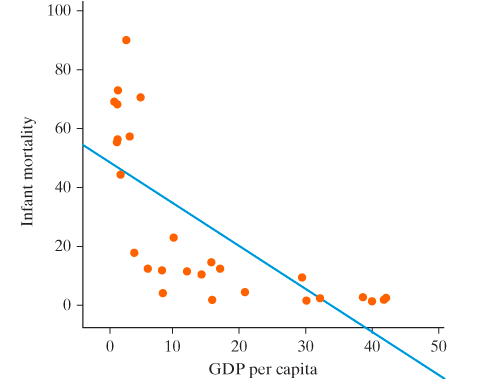
\includegraphics[keepaspectratio, width=0.6\textwidth, height=0.5\paperheight]{../img/scatter_GDP_mort}

\vspace{8pt}
{\small A real relationship. Does growth reduce infant mortality?\\ Does health drive growth? Does something else drive both?}

\end{frame}
% ----------------------------------------------------
\note{Last week ended here. The relationship is real and well measured, and the plot cannot choose between the three stories.

Today is about what it would take to choose. The short answer: a comparison in which the only relevant difference between groups is the cause you care about. The rest of the session is how to get there, and how it goes wrong.}

% ====================================================
\section{Explaining, not predicting}
% ====================================================

% ----------------------------------------------------
\begin{frame}
\frametitle{Predicting is not explaining}
\centering

\begin{itemize}[<+->]
  \item \textbf{Prediction}: given what I observe, what will I see?
  \begin{itemize}
    \item needs a stable relationship, not a causal one
    \item the rooster crowing predicts sunrise very well
  \end{itemize}
  \vspace{8pt}
  \item \textbf{Explanation}: if I \textit{change} X, what happens to Y?
  \begin{itemize}
    \item needs a model of how the world works
  \end{itemize}
  \vspace{8pt}
  \item A model can predict perfectly and be useless for intervening
\end{itemize}

\vspace{6pt}
\uncover<3->{{\footnotesize \asher{Hofman, Sharma \& Watts (2017), \textit{Science} 355(6324).}}}

\end{frame}
% ----------------------------------------------------
\note{The triad again, sharpened. Prediction needs no identification at all, which is exactly why it cannot answer a causal question.

Examples to make it concrete: Blumenstock from week 1 predicts wealth from phone records very well, and giving someone more phone credit will not make them richer. Ice-cream sales predict drownings; banning ice cream saves nobody.

For this cohort, the practical point: a model with excellent out-of-sample accuracy is evidence about prediction. It is not evidence about what would happen under an intervention, and ``feature importance'' is not a causal effect. Several of them will be tempted to write exactly that in their essays.}

% ----------------------------------------------------
\begin{frame}
\frametitle{Two languages for causality}
\centering

\begin{itemize}
  \item No brute-force way into causal inference. Two frameworks:
  \vspace{8pt}
  \item[1.] \textbf{Potential outcomes} (Rubin)
  \begin{itemize}
    \item what would have happened otherwise? Closer to experiments, economics
  \end{itemize}
  \vspace{8pt}
  \item[2.] \textbf{Causal diagrams} (Pearl)
  \begin{itemize}
    \item what causes what? Closer to observational data, epidemiology
  \end{itemize}
  \vspace{8pt}
  \item<2-> We use both, and only as far as \textbf{design} needs them
\end{itemize}

\end{frame}
% ----------------------------------------------------
\note{They will meet both in the causal inference course, with the formal apparatus. Here they are two thinking tools: potential outcomes to define what we want, diagrams to reason about what gets in the way.

Say explicitly that there will be no estimation today. The scope line for the whole course: what variation a design uses and what has to be true for it to work.}

% ====================================================
\section{Potential outcomes}
% ====================================================

% ----------------------------------------------------
\begin{frame}
\frametitle{What does ``X causes Y'' mean?}
\centering

\begin{itemize}[<+->]
  \item Not that X is the only cause of Y
  \item But that \textbf{changing X would change Y}
  \vspace{8pt}
  \item How could we see that? Repeat history, with and without X
  \vspace{8pt}
  \item The \textbf{fundamental problem of causal inference}: we can't
  \begin{itemize}
    \item $Y(1)$: the outcome if treated. $Y(0)$: the outcome if not
    \item for each unit, we see \textbf{either} $Y(1)$ \textbf{or} $Y(0)$, never both
  \end{itemize}
\end{itemize}

\end{frame}
% ----------------------------------------------------
\note{The single most important idea in the session, and it is simple enough to be undersold. Slow down.

A causal effect is a comparison between two worlds, and one of them never happens. So causal inference is a \textbf{missing data problem}: the missing value is the counterfactual. Everything else today is a strategy for filling it in with something credible.}

% ----------------------------------------------------
\begin{frame}
\frametitle{Potential outcomes framework}
\centering

\begin{itemize}
  \item Also called Neyman–Rubin causal model
  \item An effect is the difference between the \textit{actual world} and an \textit{alternative reality} (counterfactual)
  \begin{itemize}
    \item Causal effect of $X$, is $E(Y|X = 1)$ - $E(Y|X = 0)$
  \end{itemize}
\end{itemize}

\end{frame}
% ----------------------------------------------------
\note{Same idea in one line: the effect is the gap between what happened and what would have happened otherwise. The second term is the one we never see.}

% ----------------------------------------------------
\begin{frame}
\frametitle{What is the effect of smoking on Gary?}
\centering

\begin{minipage}{0.64\textwidth}
\begin{itemize}
  \item<1-> Gary smokes, doesn't exercise, is vegetarian. We can wait and see how long he lives
  \vspace{8pt}
  \item<2-> The effect of smoking on Gary: compare with a Gary who is \textit{identical except} for smoking
  \vspace{8pt}
  \item<3-> That Gary does not exist
  \vspace{8pt}
  \item<4-> Causal inference is about finding the best available stand-in for him
\end{itemize}
\end{minipage}\hfill
\begin{minipage}{0.33\textwidth}\centering
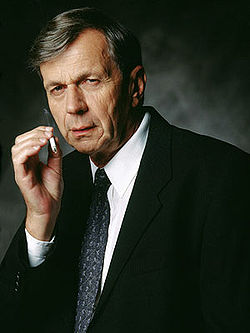
\includegraphics[width = 0.8\textwidth]{../img/smoking_man}\\{\small Gary}
\end{minipage}

\end{frame}
% ----------------------------------------------------
\note{The counterfactual Gary is the whole idea in one picture. Ask: who would you choose as a stand-in? Gary's brother? A non-smoking neighbour of the same age? Gary before he started?

Each answer is a different research design, and each has a way of failing. The brother shares genes but chose not to smoke for some reason; the neighbour differs in a hundred ways; Gary-before is younger. That is the preview for next week, where each design template is a different choice of stand-in.}

% ----------------------------------------------------
\begin{frame}
\frametitle{Potential outcomes framework}
\centering

\begin{itemize}
  \item That would be for Gary. What about the \textbf{`general' effect of smoking}?
  \item We'd need to find an alternative for every person (smoking and non-smoking), and just calculate the difference between the alternative and the reality:
  \item[] $E[LifeExp_{i}^{1}] - E[LifeExp_{i}^{0}]$
  \item[] which would be the \textbf{Average Treatment Effect} (or \textbf{ATE})
  \item<2-> Problem is we have missing data: we don't have $E[LifeExp_{i}^{1}]$ for non-smokers, and we don't have $E[LifeExp_{i}^{0}]$ for smokers
\end{itemize}

\end{frame}
% ----------------------------------------------------
\note{}

% ----------------------------------------------------
\begin{frame}
\frametitle{Potential outcomes framework}
\centering

\begin{itemize}
  \item<1-> Same goes with other quantities of interest we'll see:
  \item<2-> \textbf{ATT}, or \textbf{average treatment effect on the treated}:
  \item[]<2-> $E[Y_{i}^{1}|D_{i} = 1] - E[Y_{i}^{0}|D_{i} = 1]$
  \item[]<2-> {\small (effect of smoking among smokers)}
  \item<3-> Or the \textbf{ATC} (or ATU), or \textbf{average treatment effect on the untreated}:
  \item[]<3-> $E[Y_{i}^{1}|D_{i} = 0] - E[Y_{i}^{0}|D_{i} = 0]$
  \item[]<3-> {\small (effect of smoking among non-smokers)}
  \item[]<4->
  \item<4-> When is $ATT \neq ATC$? {\footnotesize (Non-linearity, sampling bias)}
\end{itemize}

\end{frame}
% ----------------------------------------------------
\note{}

% ----------------------------------------------------
\begin{frame}
\frametitle{PO example}
\centering

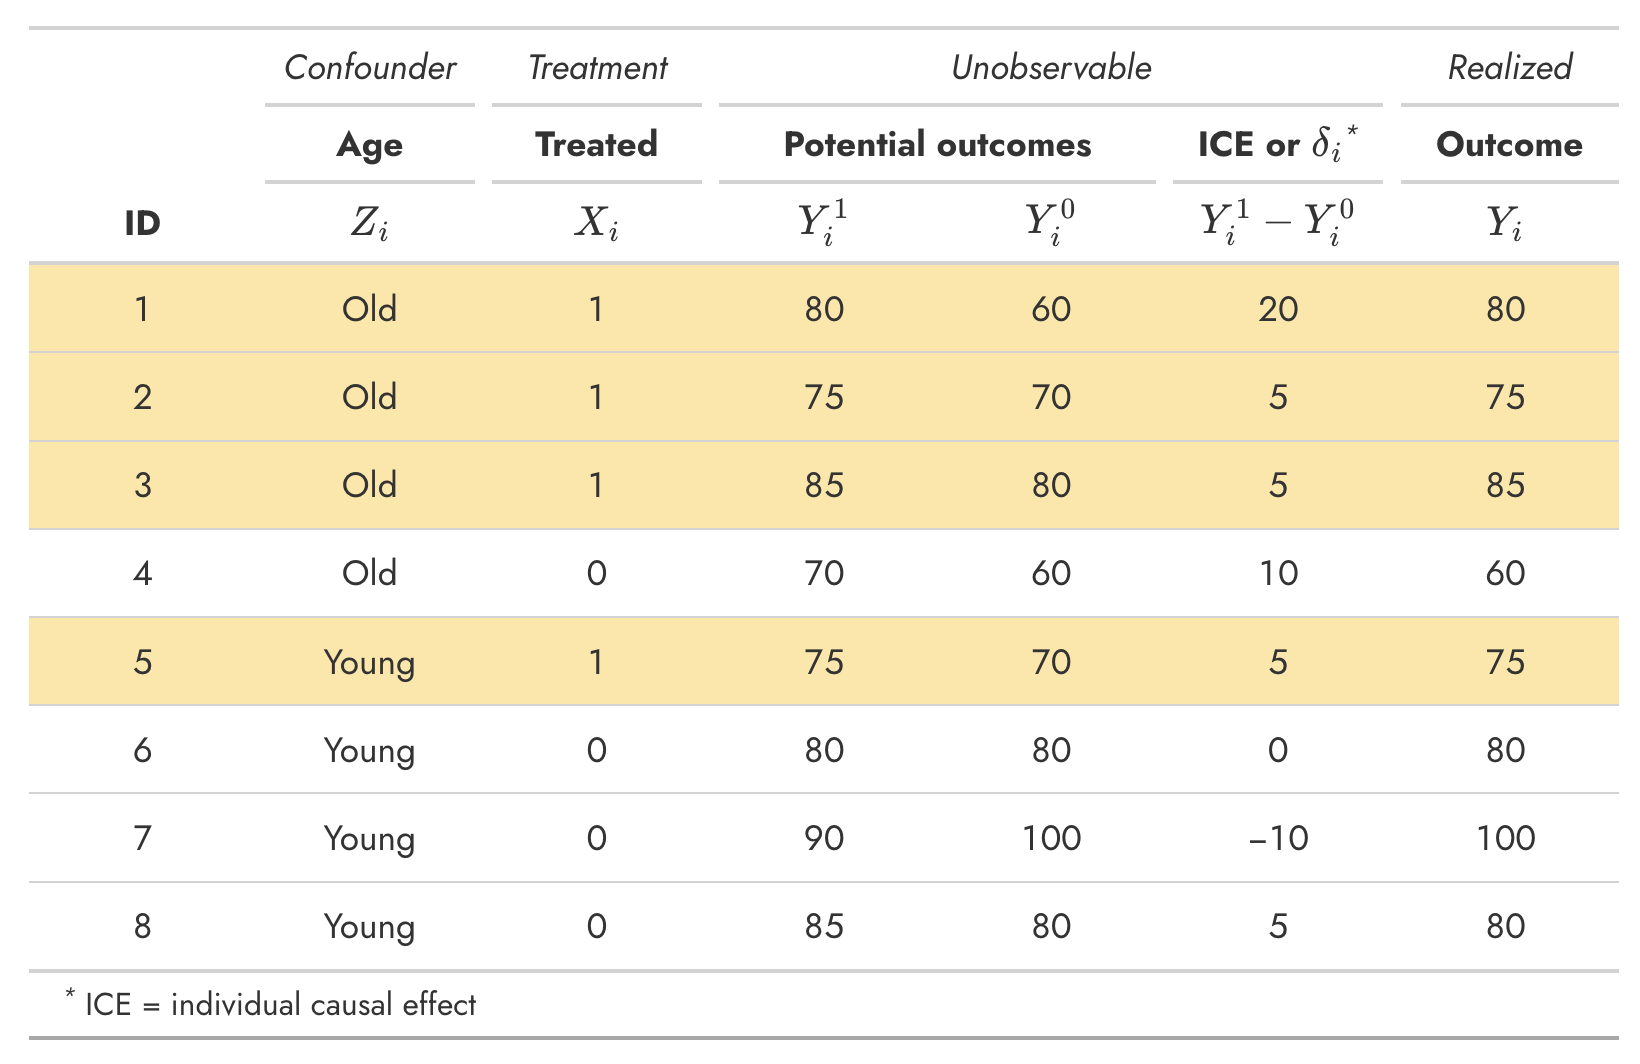
\includegraphics[width = \textwidth]{../img/po_table}

\href{https://www.andrewheiss.com/blog/2024/03/21/demystifying-ate-att-atu/}{\footnotesize https://www.andrewheiss.com/blog/2024/03/21/demystifying-ate-att-atu/}

\end{frame}
% ----------------------------------------------------
\note{}

% ----------------------------------------------------
\begin{frame}
\frametitle{PO example}
\centering

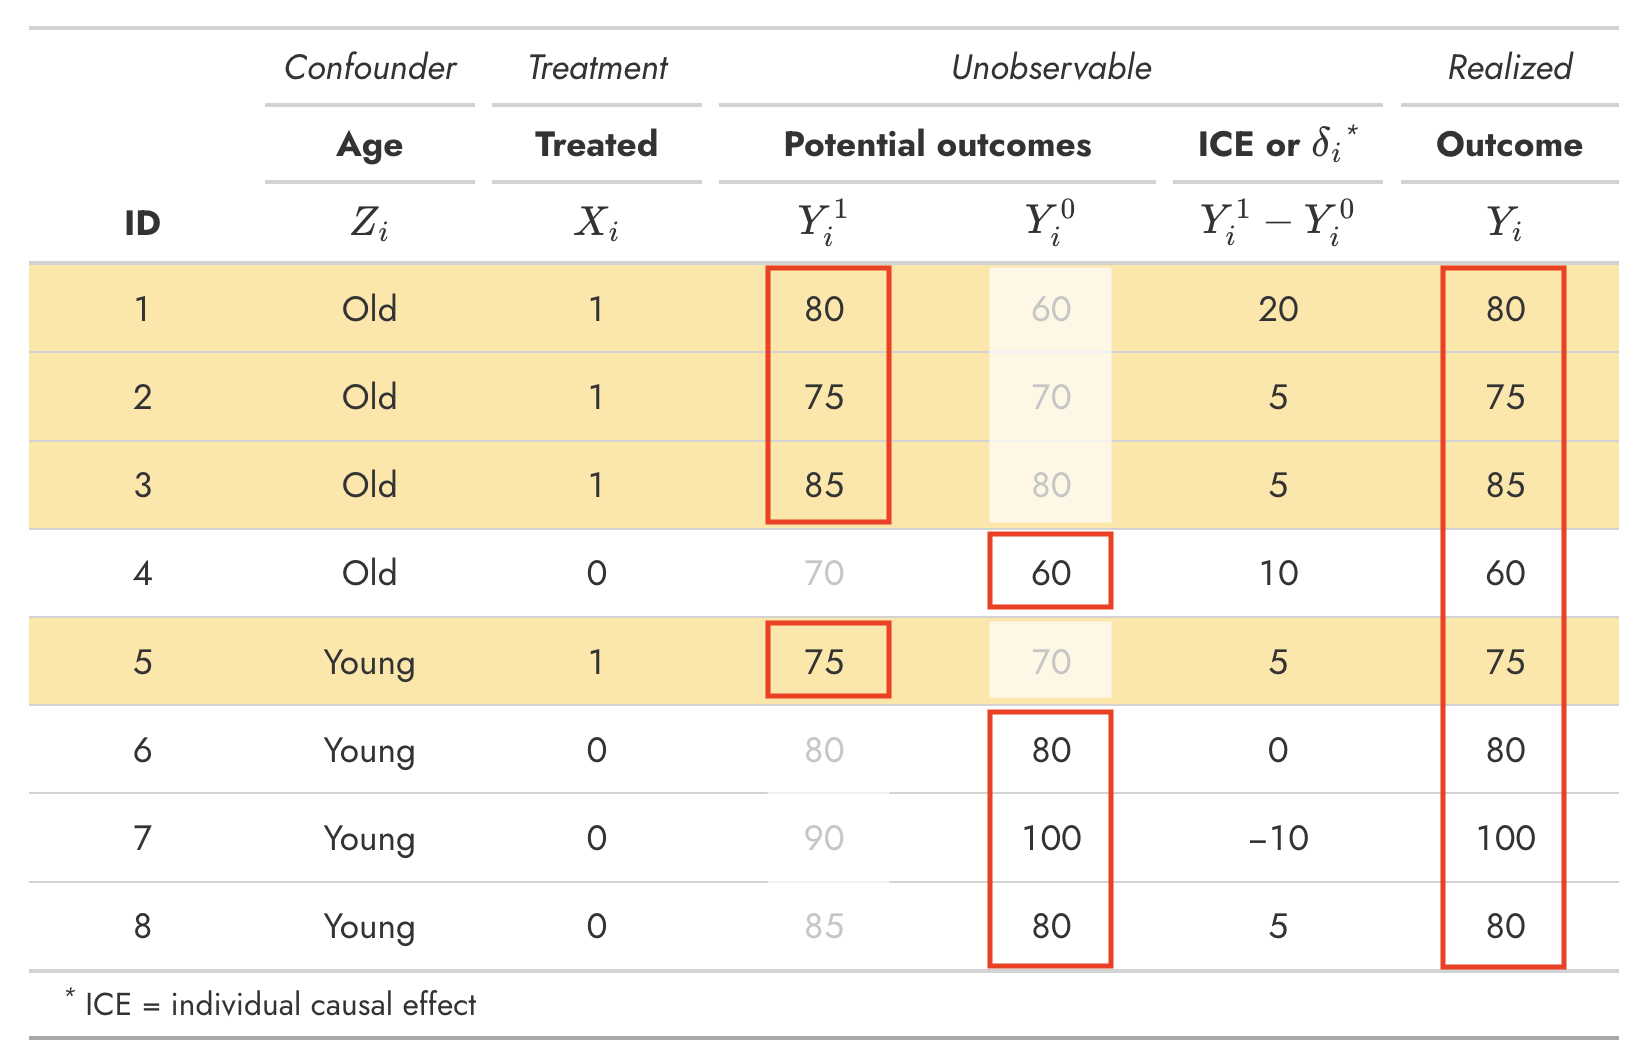
\includegraphics[width = \textwidth]{../img/po_table2}

\href{https://www.andrewheiss.com/blog/2024/03/21/demystifying-ate-att-atu/}{\footnotesize https://www.andrewheiss.com/blog/2024/03/21/demystifying-ate-att-atu/}

\end{frame}
% ----------------------------------------------------
\note{}

% ----------------------------------------------------
\begin{frame}
\frametitle{PO example}
\centering

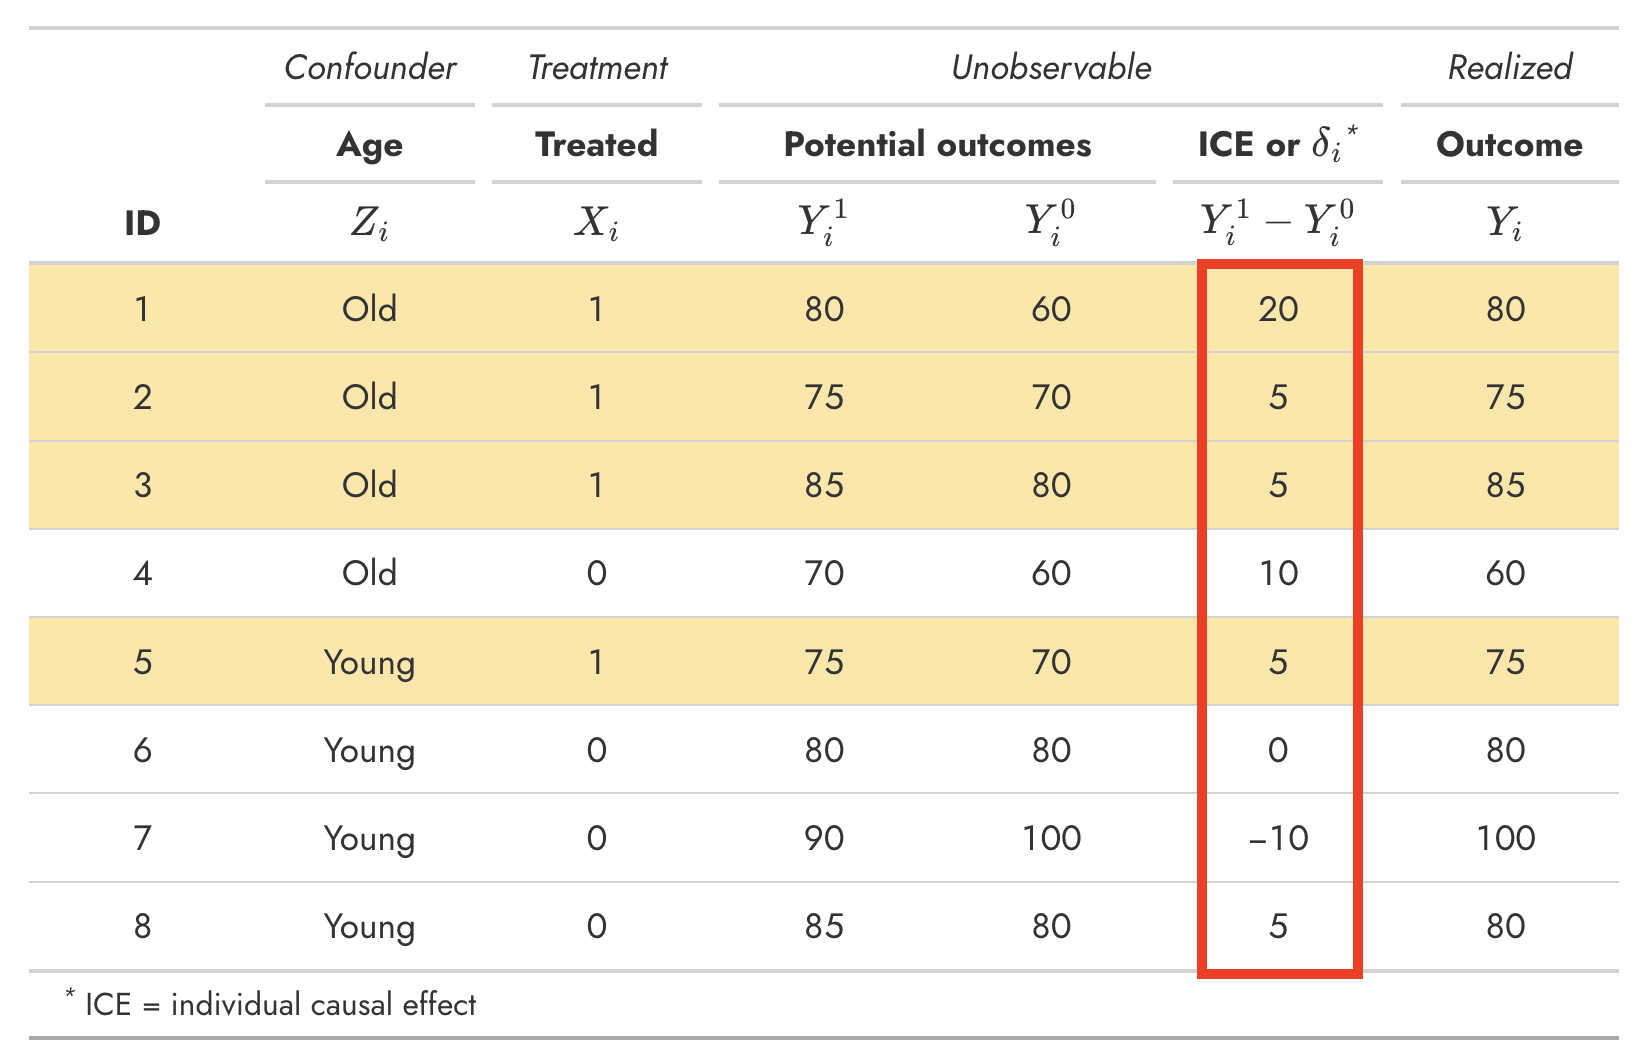
\includegraphics[width = 0.95\textwidth]{../img/po_table_ate}

$ATE = mean(20, 5, 5, 10, 5, 0, -10, 5) = 5$

\end{frame}
% ----------------------------------------------------
\note{}

% ----------------------------------------------------
\begin{frame}
\frametitle{PO example}
\centering

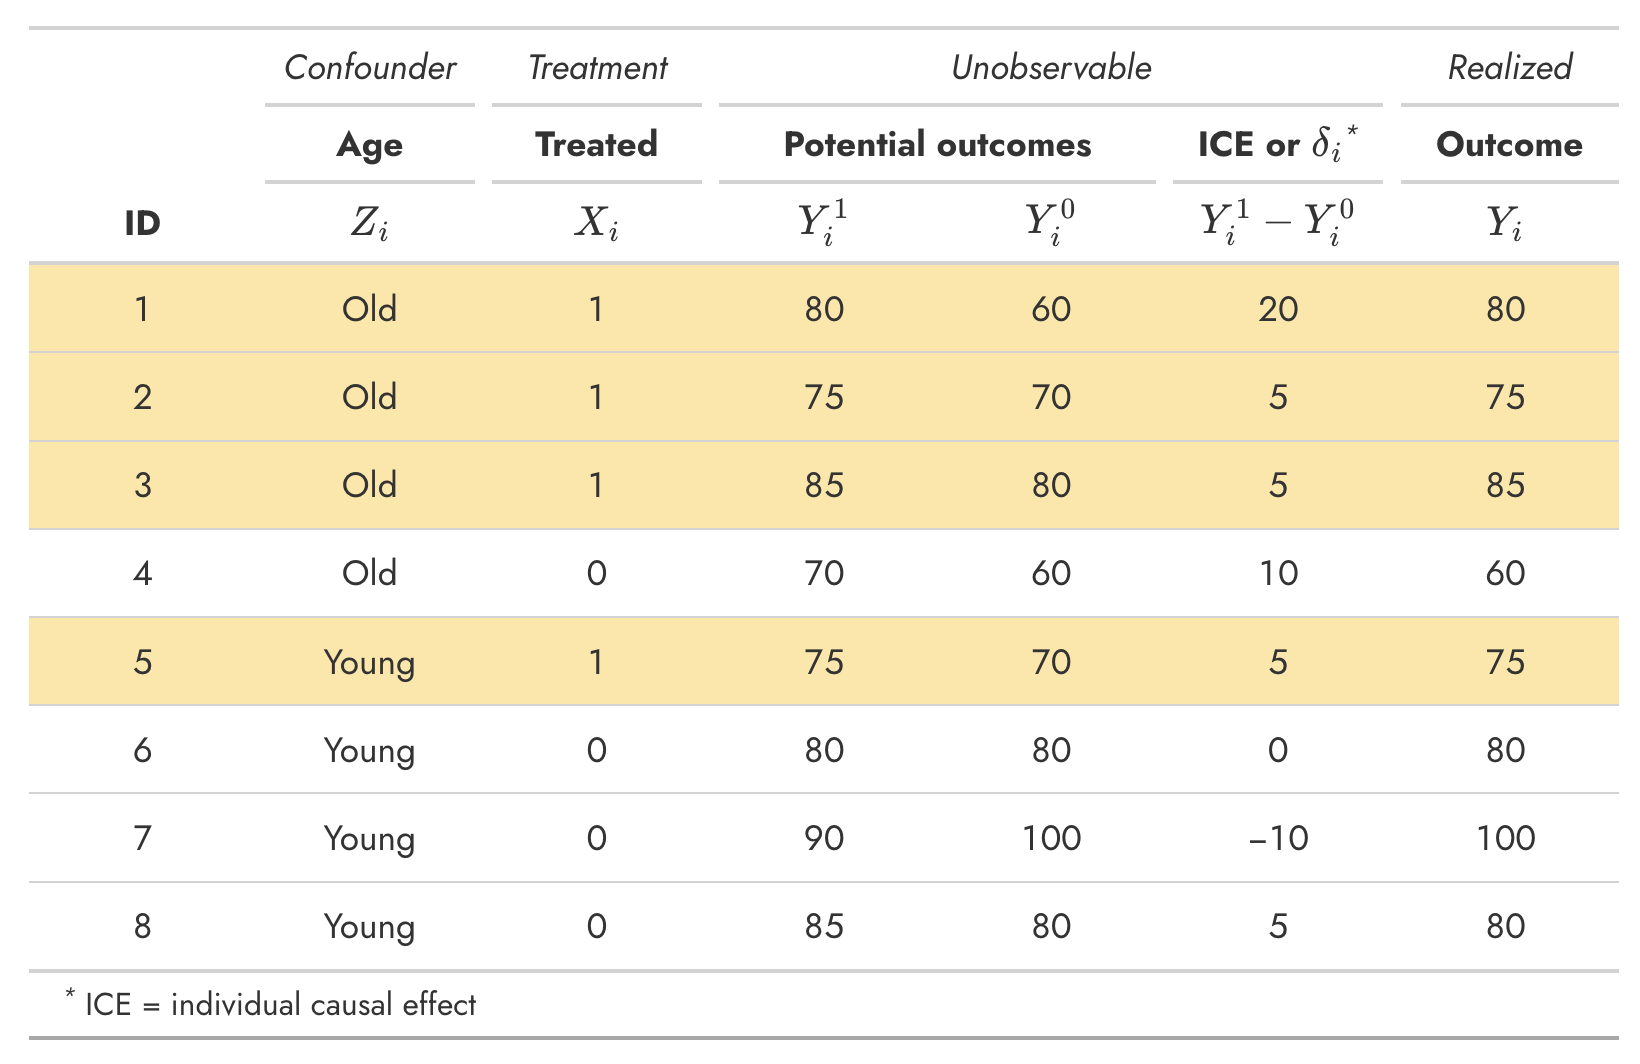
\includegraphics[width = 0.95\textwidth]{../img/po_table_att}

$ATT = mean(20, 5, 5, 5) = 8.75$

\end{frame}
% ----------------------------------------------------
\note{}

% ----------------------------------------------------
\begin{frame}
\frametitle{PO example}
\centering

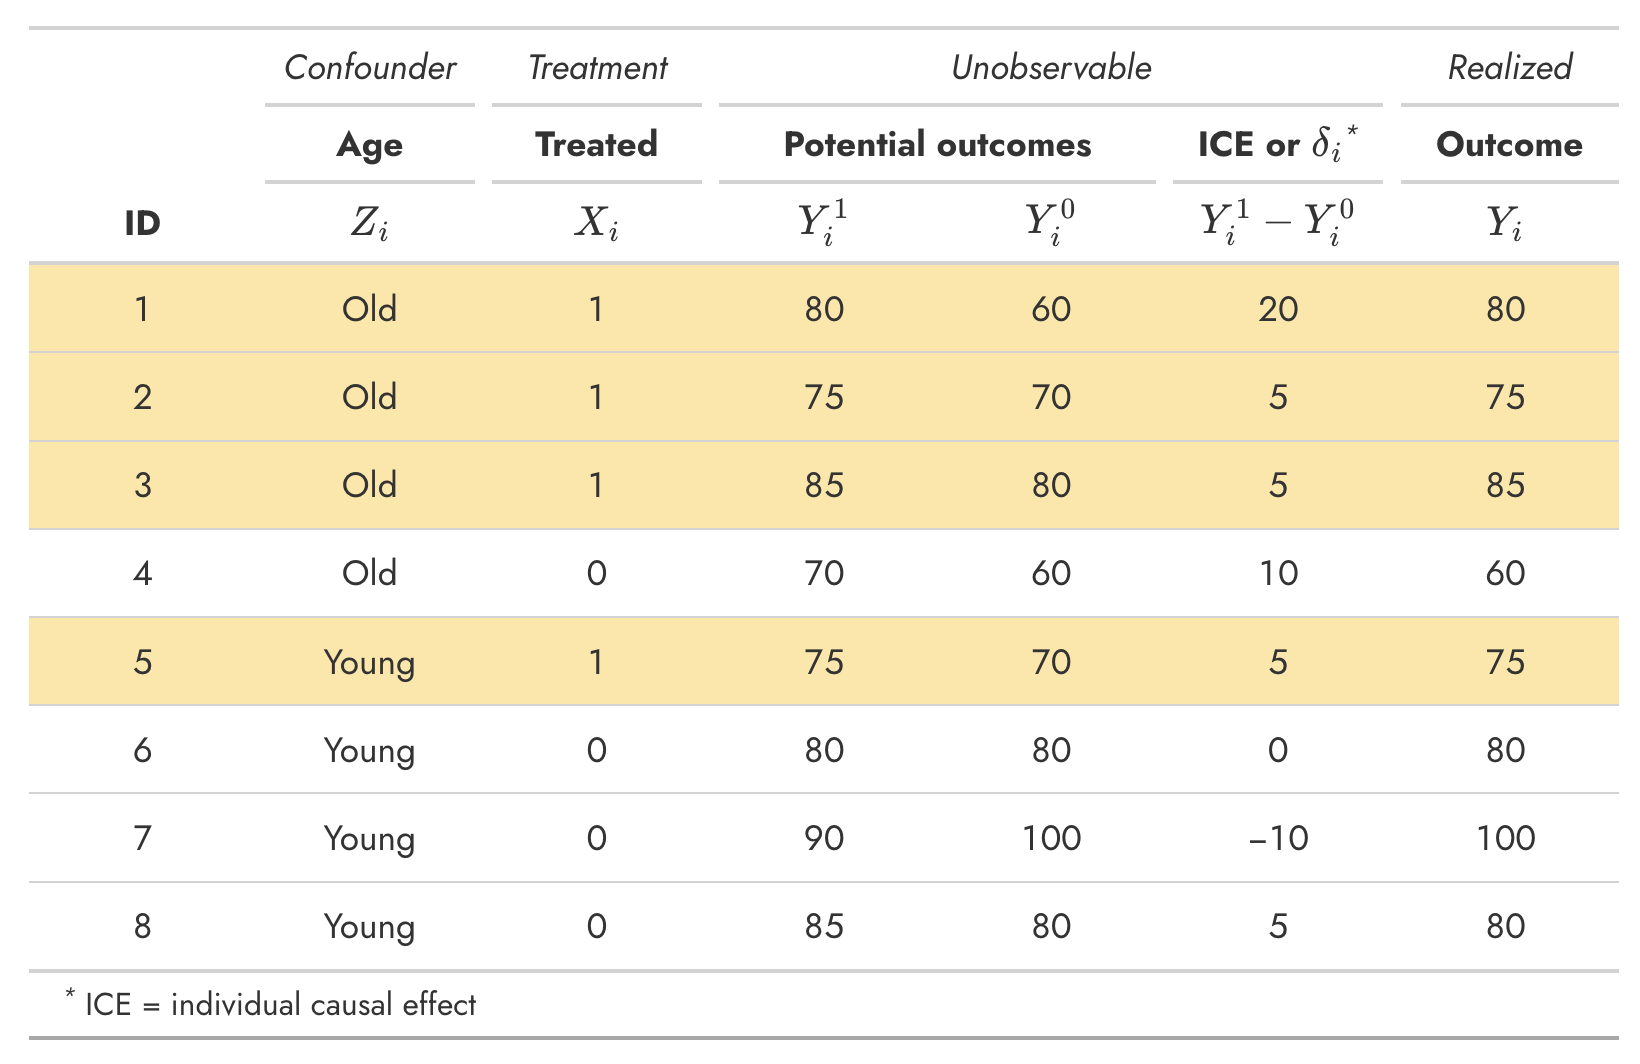
\includegraphics[width = 0.95\textwidth]{../img/po_table_atu}

$ATU = mean(10, 0, -10, 5) = 1.25$

\end{frame}
% ----------------------------------------------------
\note{}

% ----------------------------------------------------
\begin{frame}
\frametitle{PO example}
\centering

\begin{itemize}
  \item Weighted mean of ATT and ATU $=$ ATE
  \item But we \BGyellow{don't have both} $Y_{0}$ and $Y_{1}$
  \item Two ways of looking into this observationally
  \begin{itemize}
    \item (assuming \textbf{age} as the \BGyellow{only} confounder)
  \end{itemize}

\end{itemize}

\end{frame}
% ----------------------------------------------------
\note{}

% ----------------------------------------------------
\begin{frame}
\frametitle{PO example}
\centering

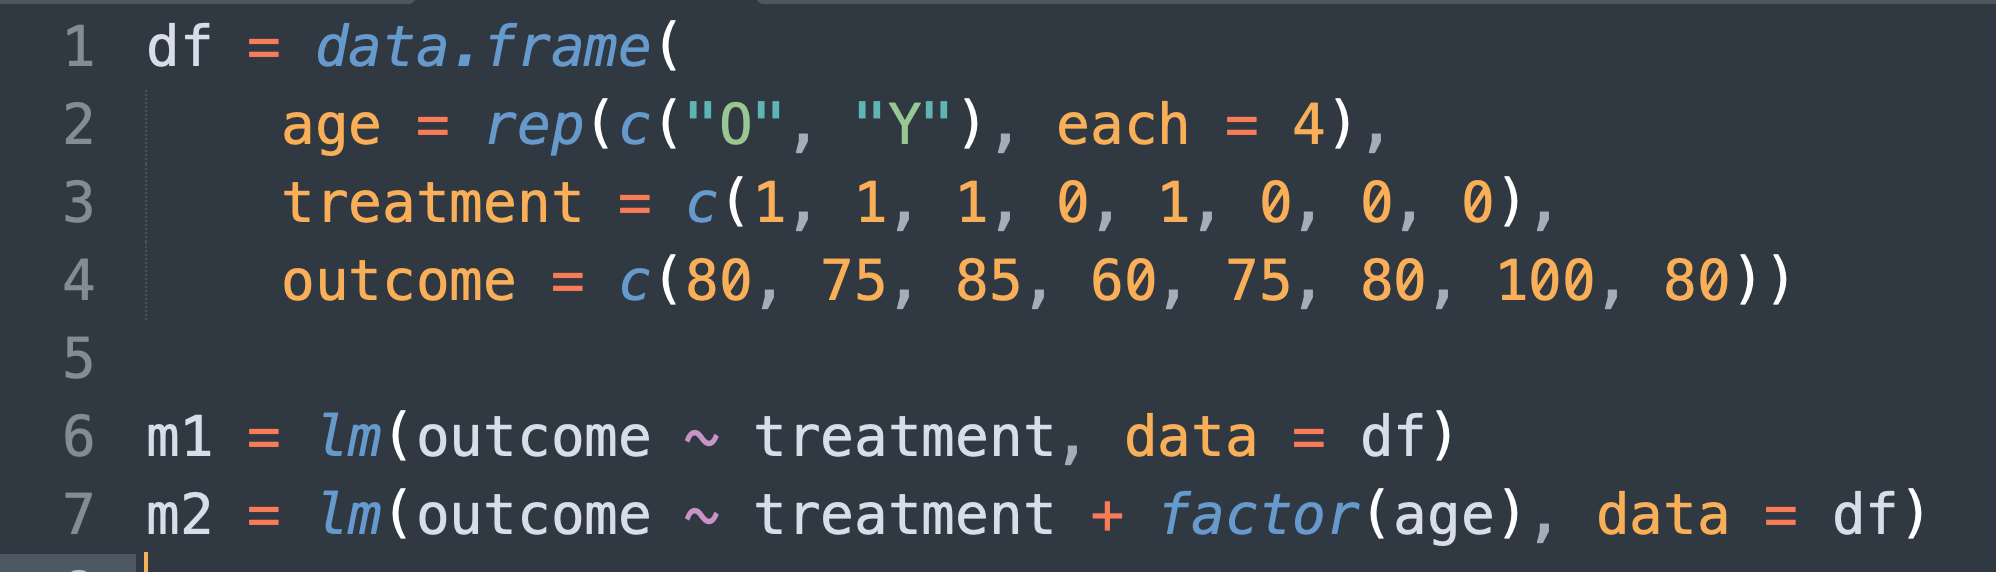
\includegraphics[width = \textwidth]{../img/po_data}

\end{frame}
% ----------------------------------------------------
\note{}

% ----------------------------------------------------
\begin{frame}
\frametitle{PO example}
\centering

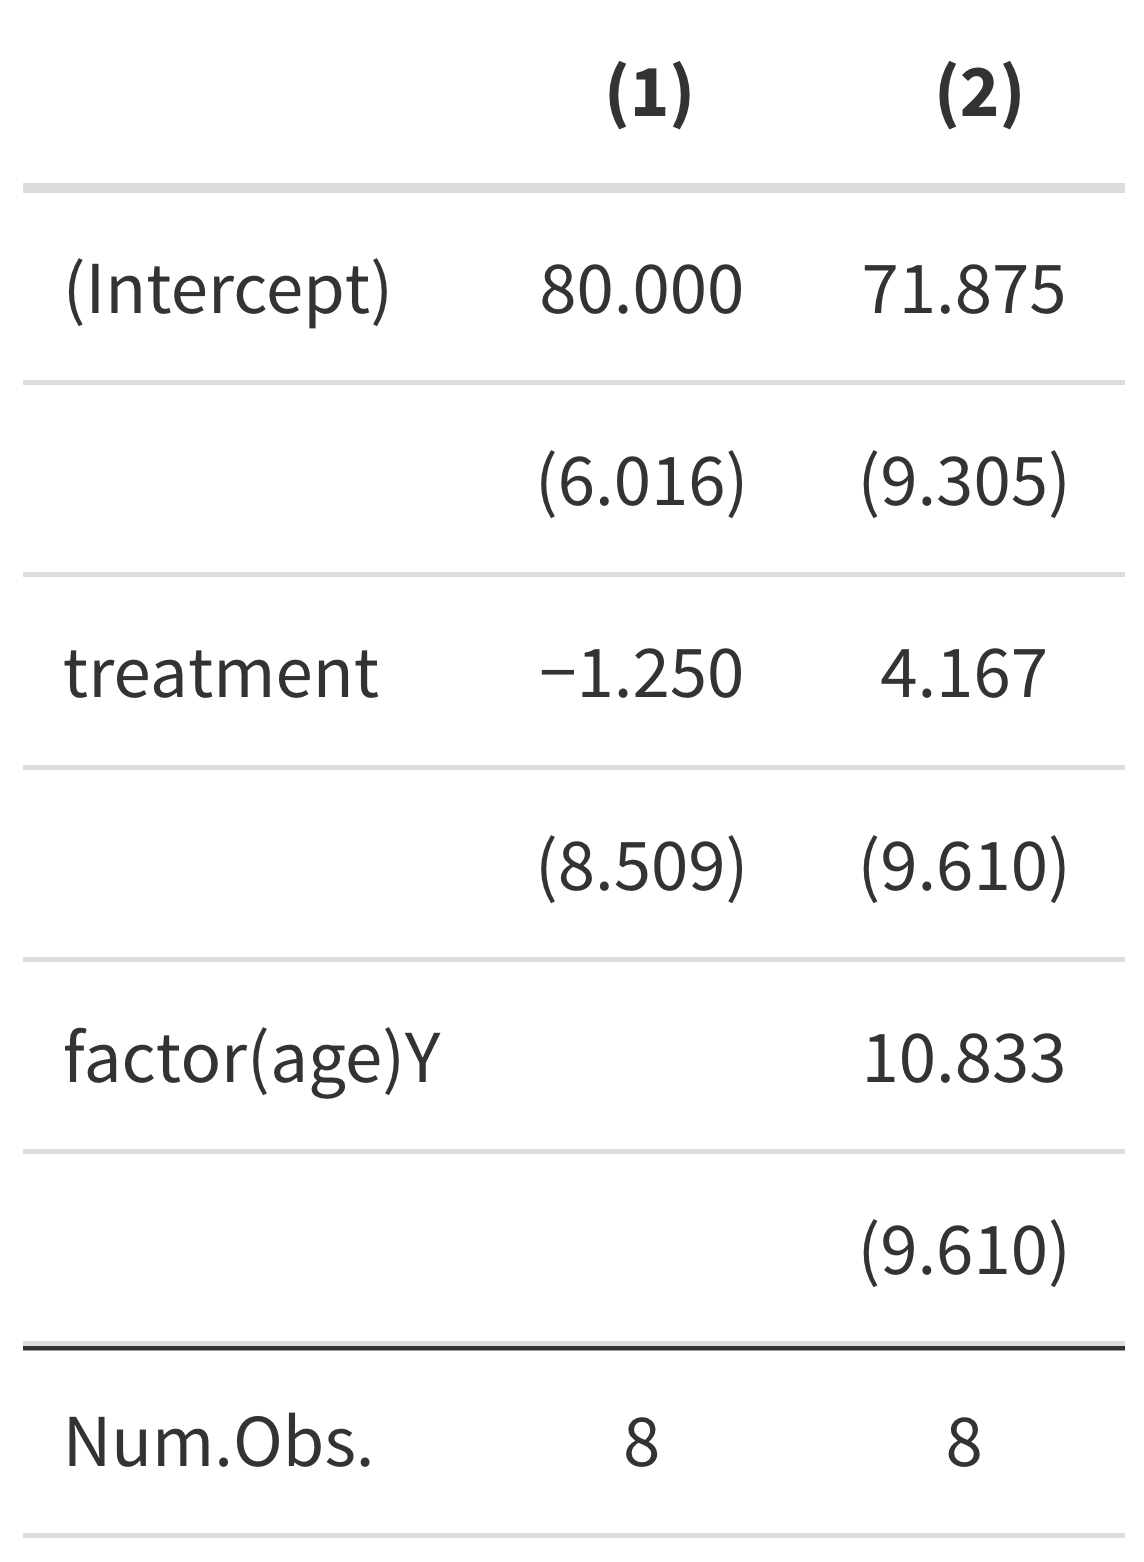
\includegraphics[width = .5\textwidth]{../img/po_regression}

\end{frame}
% ----------------------------------------------------
\note{}

% ----------------------------------------------------
\begin{frame}
\frametitle{Sometimes ATT is more useful in practice}
\centering

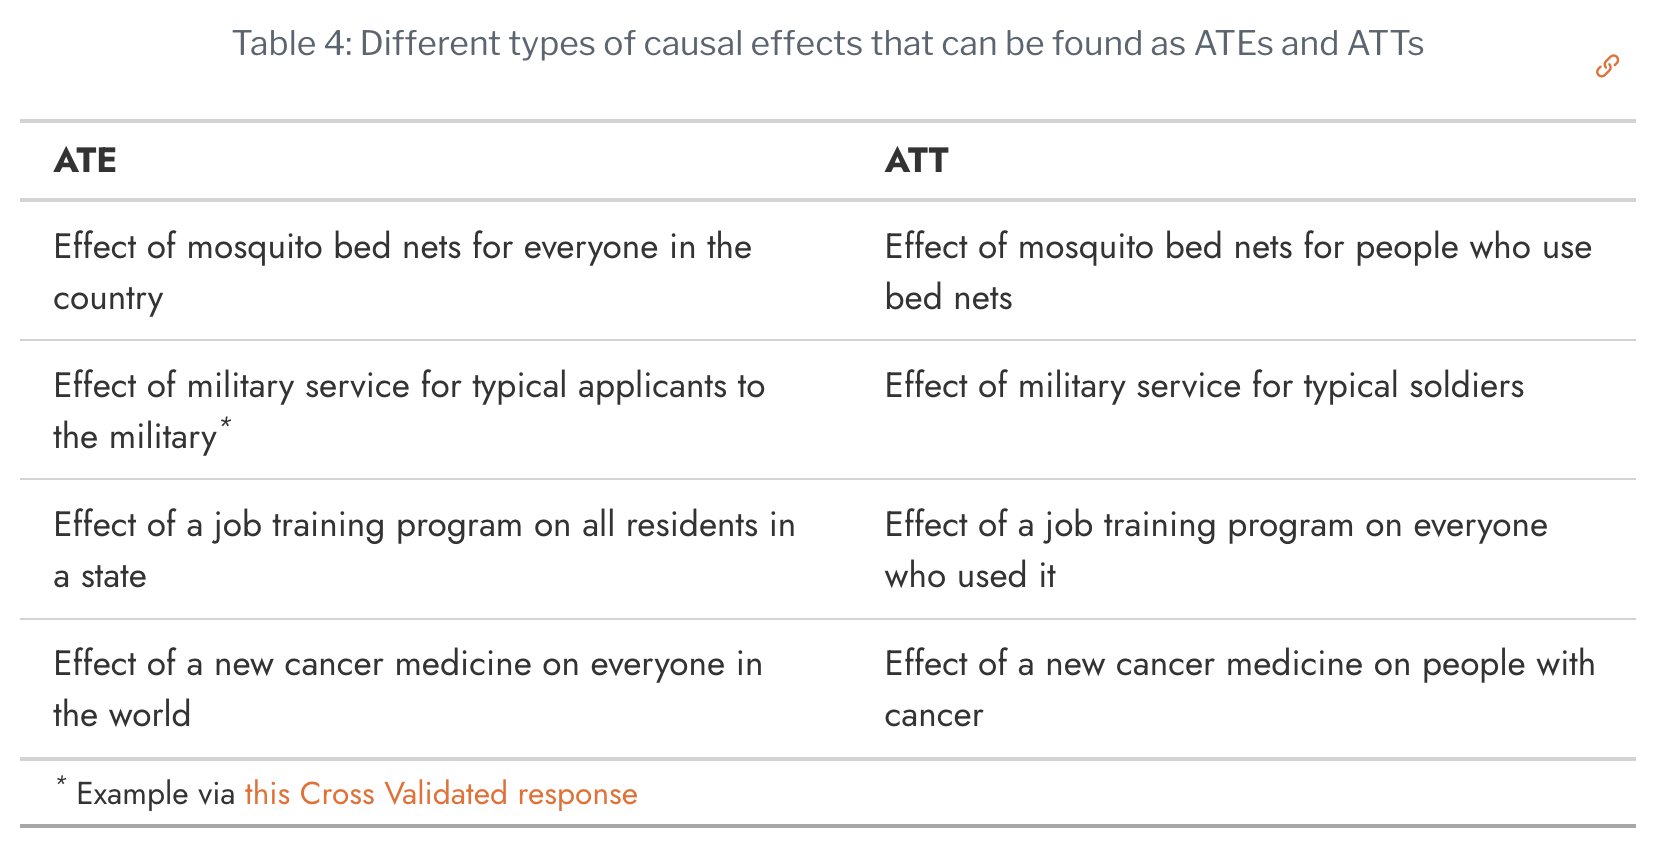
\includegraphics[width = \textwidth]{../img/ate_att}

\href{https://www.andrewheiss.com/blog/2024/03/21/demystifying-ate-att-atu/}{\footnotesize https://www.andrewheiss.com/blog/2024/03/21/demystifying-ate-att-atu/}

\end{frame}
% ----------------------------------------------------
\note{}

% ====================================================
\section{Experiments}
% ====================================================

% ----------------------------------------------------
\begin{frame}
\frametitle{Estimating causal effects}
\centering

\begin{itemize}
  \item \textbf{So how do we solve this missing data problem?}
  \begin{itemize}
    \item intervening in treatment assignment through randomization
  \end{itemize}
  \item[]
  \item<2-> `No causation without manipulation' (Rubin)
  \item<2-> Potential outcomes framework initially developed for \textit{experimental data}: randomized controlled trials are the gold-standard in approximating the alternative reality (counterfactual)
  \item<2-> But there are also problems or limitations:
  \begin{itemize}
    \item issues in experimental design (next)
    \item more importantly: not all experiments are feasible or ethical
  \end{itemize}
\end{itemize}

\end{frame}
% ----------------------------------------------------
\note{}

% % ----------------------------------------------------
% \begin{frame}
% \frametitle{Issues in experimental designs}
% \centering
%
% \begin{itemize}
%   \item[] Experiments also have their problems, e.g.:
%   \item Non-perfect randomization (esp. if block-r)
%   \item SUTVA (or stable unit treatment value assumption)
%   \item Attrition
%   \item Treatment compliance (estimating the intent-to-treat, or ITT)
%   \item External validity
%   \item etc
% \end{itemize}
%
% \end{frame}
% % ----------------------------------------------------

% ----------------------------------------------------
\begin{frame}
\frametitle{Randomization issues}
\centering

\begin{itemize}
  \item Obviously, the basic of any experiment is that \textbf{treatment assignment is random}
  \item It's not frequent, but could happen that this randomization is not well done
  \item Also it might not let us detect the effect, and having statistical issues, especially when using \textit{block} randomization, or \textit{unit} vs. \textit{cluster} randomization
  \item[]
  \item Also could be an issue when doing \textit{block randomization}
\end{itemize}

\end{frame}
% ----------------------------------------------------
\note{}

% ----------------------------------------------------
\begin{frame}
\frametitle{SUTVA}
\centering

\begin{itemize}
  \item SUTVA stands for \textbf{Stable Unit Treatment Value Assumption}, and it is a key assumption in experimental designs
  \begin{itemize}
    \item It is basically that the outcome in one unit is \textbf{not} affected by treatment assignment in other units
  \end{itemize}
  \item Diffusion effects among subjects?
  \begin{itemize}
    \item One solution could be to think about \textit{unit of observation}
  \end{itemize}
  \item (This problem is also discussed in causal inference with observational data)
\end{itemize}

\end{frame}
% ----------------------------------------------------
\note{}

% ----------------------------------------------------
\begin{frame}
\frametitle{Attrition}
\centering

\begin{itemize}
  \item \textbf{Attrition} is just the case when `participants leave the study'
  \item More generally, when some of the units in the experiment do not complete it
  \item The key question is, to what extent is this biasing the results?
\end{itemize}

\end{frame}
% ----------------------------------------------------
\note{}

% ----------------------------------------------------
\begin{frame}
\frametitle{External validity}
\centering

\begin{itemize}
  \item To what extend can we \textbf{generalize the results of an experiment}?
  \begin{itemize}
    \item i.e., how much do we really learn with this experiment?
  \end{itemize}
  \item This is a more general issue that we will also discuss with observational-data studies, but perhaps very relevant for experiments because of the setting it usually takes place
  \item Example: media exposure studies (or Guess \textit{et al} 2023)
  \begin{itemize}
    \item \BGyellow{Treatment validity?} Discuss concept of \textbf{bundled treatment}
    \item \BGyellow{Outcome validity?} survey (hypothetical) questions vs behavioral outcomes, relationship with original Q
  \end{itemize}
\end{itemize}

\end{frame}
% ----------------------------------------------------
\note{}

% ----------------------------------------------------
\begin{frame}
\frametitle{Treatment compliance}
\centering

\begin{itemize}
  \item Are all units assigned to treatment really exposed to it?
  \item In clinical trials, e.g. do they take the pill or spit it?
  \item How would this look like in an experiment when you pay (treated) individuals to watch TV or use Facebook?
  \item Concept of \textbf{intention-to-treat} (ITT) analyses and the \textbf{complier average causal effect} or \textbf{local average treatment effect} (LATE)
\end{itemize}

\end{frame}
% ----------------------------------------------------
\note{}

% ====================================================
\section{Causal models and diagrams}
% ====================================================

% ----------------------------------------------------
\begin{frame}
\frametitle{So how to we approximate $Y^{0}$?}
\centering

\begin{itemize}
  \item Experiments are fine, but often not possible
  \item<2-> How do we do this with \textbf{observational data}?,
    \begin{itemize}
      \item We need to `build' a counterfactual
    \end{itemize}
  \item<3-> Basic idea: we come up with a strategy where the only variation we analyze is (according to us) \textit{due} to the independent variable (cause) we are interested in
  \begin{itemize}
    \item \textbf{Read it again:} it is actually the same idea as in the experimental method, where we use randomization to achieve that
  \end{itemize}
  \item<4-> But in order to do that, we need to be clear about the \textbf{causal model} that is causing $Y$, so we know what we need to control for
  \begin{itemize}
    \item And we're gonna use \BGyellow{causal diagrams} for that
  \end{itemize}
\end{itemize}

\end{frame}
% ----------------------------------------------------
\note{}

% ----------------------------------------------------
\begin{frame}
\frametitle{Example}
\centering

\begin{itemize}
\item Let's say we want to know whether a cleaner environment makes people happier
\end{itemize}

\end{frame}
% ----------------------------------------------------
\note{}

% ----------------------------------------------------
\begin{frame}
\frametitle{Example}
\centering

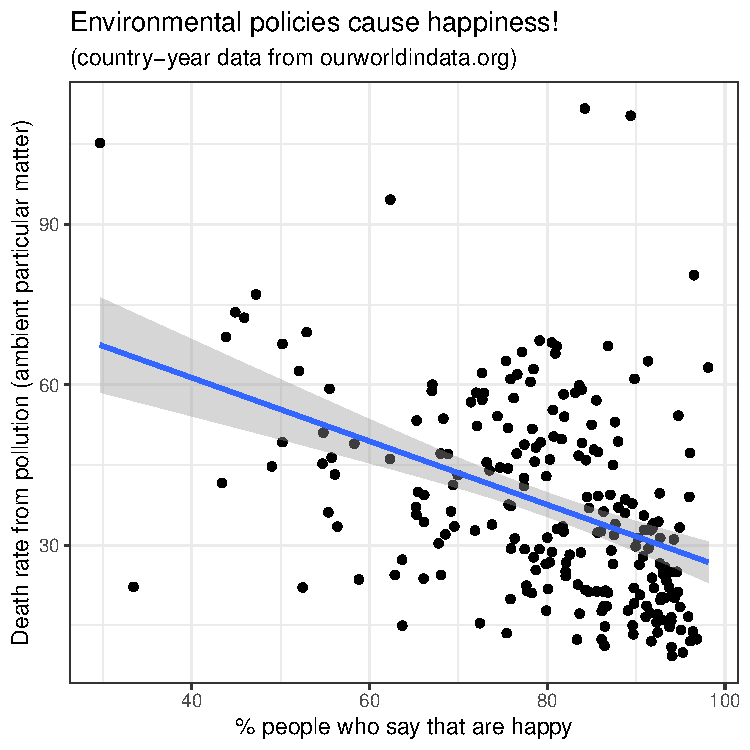
\includegraphics[width = 0.65\textwidth]{../img/happiness_pollution}

\end{frame}
% ----------------------------------------------------
\note{}
% ----------------------------------------------------
\begin{frame}
\frametitle{Example}
\centering

\begin{itemize}
  \item Remember that out problem (the `fundamental problem of causal inference` etc) is that we can observe these countries but not their \textbf{alternatives} without treatment (or with different levels of the treatment)
  \item So to infer causal models we need to \textbf{isolate the variation due to our treatment}, how?
  \begin{itemize}
    \item Controlling the non-causal variation
  \end{itemize}
  \item To get to this, we need to have a \BGyellow{causal model} to know what's `contaminating' our outcome (so we know what we should be controlling for)
\end{itemize}

\end{frame}
% ----------------------------------------------------
\note{}

% ----------------------------------------------------
\begin{frame}<handout:4>
\frametitle{Our causal model}
\centering

\begin{tikzpicture}[every text node part/.style={align=center}, scale = 0.75]

% Process

\node (ep) at (0,0){Cleaner environment};
\node (h) at (7,0){Happiness};
\only<1|handout:1>{\draw[->] (ep) -- (h);}
\only<1|handout:1>\node[color=white] (m) at (3.5,3){Wealth};
\only<2-|handout:2->\node (m) at (3.5,3){Wealth};
\only<4|handout:4>\node (z) at (6,2.75){Z};
\only<2|handout:2>\draw[->] (m) -- (h);
\only<2-4|handout:2-4>\draw[->] (m) -- (ep);
\only<2|handout:2>{\draw[->, solid] (ep) -- (h);}
\only<3-|handout:3->{\draw[->] (ep) -- (h);}
\only<4|handout:4>\draw[->] (m) -- (z);
\only<4|handout:4>\draw[->] (z) -- (h);
\only<5|handout:5>\draw[->] (m) -- (3.5, 0);

\end{tikzpicture}

\vspace{20pt}

\begin{itemize}
  \only<1|handout:1>{\item This is our initial causal model: having a cleaner environment makes people happier (because they like looking into a blue sky without smog), and that's it. We do not have to control for anything nor do anything else.}
  \only<2|handout:2>{\item Wait, but maybe it's about money, isn't it? Actually, wealthier countries tend to have cleaner environments and, at the same time, money causes happiness. \textbf{We need to control for wealth.}}
  \only<3|handout:3>{\item Or perhaps is not that money increases happiness \textit{per se}, but that it does so through other \textbf{mediators}: wealth allows countries to focus on environment, which increases happiness. \textbf{Again, no need to control.} As long as this is the \textbf{only} mediator.}
  \only<4|handout:4>{\item We are happy with that model, but we're still missing something. Say we believe that money does not have any direct causal effect, but it does causes some other things (labour conditions, cultural offer, ... let's call them $Z$) and these, in turn, have an effect on happiness. \textbf{We need to control for wealth and all $Z$.}}
  \only<5|handout:5>{\item (Another thing would be if money \textbf{moderates} the relationship between environmental policies and happiness: spending resources to take care of our environment makes you happier only if you have enough money -- this is an special case, we could talk about heterogenous effects)}
\end{itemize}

\end{frame}
% ----------------------------------------------------
\note{}
% ----------------------------------------------------
\begin{frame}
\frametitle{Basics of causal inference}
\centering

\begin{itemize}[<+->]
  \item So to come up with an strategy, we need to understand what's going on in terms of the data generating process
  \begin{itemize}
    \item This applies from the most basic strategy (add controls) to the more complicated ones (e.g. evaluating DiD or RDD)
  \end{itemize}
  \item Once we have that, we can \textbf{identify} an effect (in other words: isolating the causal variation from other sources of variation we are not interested in)
\end{itemize}

\end{frame}
% ----------------------------------------------------
\note{}

% ----------------------------------------------------
\begin{frame}
\frametitle{Causal models, mechanisms, and DAGs}
\centering

\begin{itemize}
  \item We will use \BGyellow{Directed Acyclic Graphs (DAG)} (causal diagrams), a graph where we link \textbf{variables} (nodes) with \textbf{causal effects} (arrows)
  \item[]
  \item[]<2-> A few things:
  \item<3-> Only one-directional causality (\textit{acyclic})
  \begin{itemize}
    \item if you have feedback cycles, write multiple nodes for $t_{1}$, $t_{2}$
  \end{itemize}
  \item<4-> Sometimes: solid lines $\rightarrow$ observed, dashed $\rightarrow$ unobserved ($U$)
  \item<5-> Treatment usually written as $D$ (and $Y$ the outcome)
  \item<6-> Combine variables (usually $B$ for background, or $U$ for unknown)
  \item<7-> No arrow means \textit{no effect}, explicitly
\end{itemize}

\end{frame}
% ----------------------------------------------------
\note{}

% ----------------------------------------------------
\begin{frame}
\frametitle{This is a DAG}
\centering

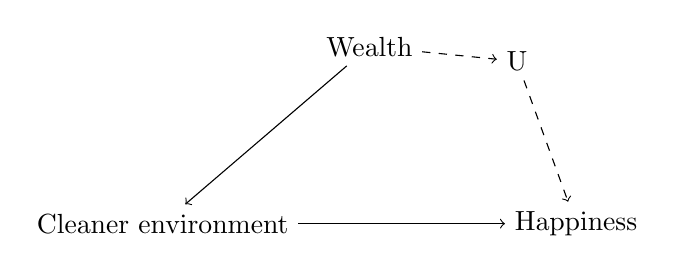
\begin{tikzpicture}[every text node part/.style={align=center}, scale = 0.75]

\node (ep) at (0,0){Cleaner environment};
\node (h) at (7,0){Happiness};
\node (z) at (6,2.75){U};
\node (m) at (3.5,3){Wealth};
\draw[->] (m) -- (ep);
\draw[->, dashed] (m) -- (z);
\draw[->, dashed] (z) -- (h);
\draw[->] (ep) -- (h);

\end{tikzpicture}

\end{frame}
% ----------------------------------------------------
\note{}
% ----------------------------------------------------
\begin{frame}
\frametitle{This is another DAG}
\centering

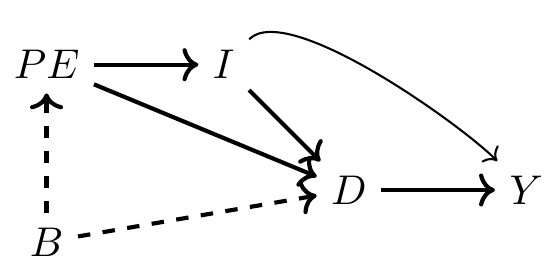
\includegraphics[width = 0.6\textwidth]{../img/dag_earnings}

\vspace{15pt}

\begin{itemize}\footnotesize
  \item Y = earnings (outcome)
  \item D = college education (treatment)
  \item PE = parental education
  \item I = family income
  \item B = unobserved background factors (intelligence, abilities, home, etc)
\end{itemize}

{\tiny from \url{https://mixtape.scunning.com/03-directed_acyclical_graphs}}

\end{frame}
% ----------------------------------------------------
\note{}

% ----------------------------------------------------
\begin{frame}
\frametitle{Causal models, mechanisms, and DAGs}
\centering

\begin{itemize}
  \item[] We use DAGs for mainly two things related to causal inference:
  \item Drawing up the \textbf{mechanism} that explains the outcome
  \item Come up with the strategy we need to \textbf{identify} the causal effect
  \item[]
  \begin{itemize}
    \item<2-> The difference between the mechanism and the causal model is that not all intermediate steps are relevant for causal inference, even though they do work as an additional check
  \end{itemize}
\end{itemize}

\end{frame}
% ----------------------------------------------------
\note{}

% ----------------------------------------------------
\begin{frame}
\frametitle{Mediation and moderation}
\centering

\begin{itemize}
\item We usually find more than one variable present in a mechanism
\item Two typical variables: mediator and moderator
\item \BGyellow{Mediation}: a third variable explains the causal relationship between two variables (e.g. flu infection $>$ immune reaction $>$ fever)
\item \BGyellow{Moderation}: a third variable changes the effect of one variable on another (e.g. how age changes the immune reaction)
\end{itemize}

\end{frame}
% ----------------------------------------------------
\note{}

% ----------------------------------------------------
\begin{frame}<handout:3>
\frametitle{Example: income inequalities}
\centering

\begin{tikzpicture}[every text node part/.style={align=center}, scale = 0.75]

% Process

\node (pe) at (0,0){Parents' education};
\node (i) at (7,0){Income (children)};
\only<1|handout:1>{\node[color=white] (e) at (5,2.5){Children's education};}
\only<1|handout:1>{\draw[->] (pe) -- (i);}

\only<2-|handout:2->{\node (e) at (6,2.5){Children's education};}
\only<2|handout:2>{\draw[->] (pe) -- (e);}
\only<2-|handout:2->{\draw[->] (e) -- (i);}
\only<2-|handout:2->{\draw[->, dashed] (pe) -- (i);}

\only<3-|handout:3->{\node (fi) at (1,2.5){Family income};}
\only<3-|handout:3->{\draw[->] (pe) -- (fi);}
\only<3-|handout:3->{\draw[->] (fi) -- (e);}

\end{tikzpicture}

\vspace{20pt}

\begin{itemize}
  \only<1|handout:1>{\item Say we want to explain income inequality, and we find that people whose parents went to university earn, on average, more. This would be the basic causal model.}
  \only<2|handout:2>{\item But \textit{why} it is so? Someone comes and says: ``It's because parents with higher education are more likely to send their children to university and help them get through.''}
  \only<3|handout:3>{\item And then someone comes and says: ``It's not only that, it's money. Parents with higher education are richer and are able to send their kids to private schools and universities.''}
\end{itemize}

\vspace{20pt}

{\footnotesize (\textit{Note:} in this case I use solid lines for direct effects and dashed lines for indirect effects, kind of)}

\end{frame}
% ----------------------------------------------------
\note{}

% ----------------------------------------------------
\begin{frame}
\frametitle{DAGs and mechanisms}
\centering

\begin{itemize}[<+->]
\item We can draw the process we're trying to study
\item Main idea: focus on the \textit{causal model}
  \begin{itemize}
  \item What had to happen for kids with university-degree parents to get richer?
  \item In other words, what mechanisms were in play behind what we see in the data?
  \end{itemize}
\item This matters when choosing our empirical strategy:
  \begin{itemize}
  \item Main identification strategy
  \item Additional checks or implications (testing the mechanism, heterogenous effects, etc)
  \end{itemize}
\end{itemize}

\end{frame}
% ----------------------------------------------------
\note{}

% ====================================================
\section{Back doors and front doors}
% ====================================================

% ----------------------------------------------------
\begin{frame}
\frametitle{Front doors and back doors}
\centering

\begin{itemize}
  \item<1-> We are interested in \textit{identifying} the effect of pollution on happiness: that's out \textbf{front door}
  \item<2-> To do so, you have to make sure that the `water flows' through this front door, and not through other `pipe', or back door
  \item[]
  \item<3-> \texttt{Pollution -> Happiness} is our front door
  \item<3-> \texttt{Pollution <- Wealth -> Happiness} is a back door
  \item<4-> How do you close it? Just controlling for \texttt{Wealth}
\end{itemize}

\end{frame}
% ----------------------------------------------------
\note{}

% ----------------------------------------------------
\begin{frame}
\frametitle{Front doors and back doors}
\centering

\begin{itemize}
  \item There are esentially two ways to do causal inference:
  \item[1.] Close all back doors and leave only the front door open
  \item[] That's where DAGs help to identify these variables
  \item[]
  \item[2.] Using some other method where only the front door is opened
  \item[] (Finding and analysing exogenous variation)
\end{itemize}

\end{frame}
% ----------------------------------------------------
\note{}

% ----------------------------------------------------
\begin{frame}
\frametitle{Front doors and back doors}
\centering

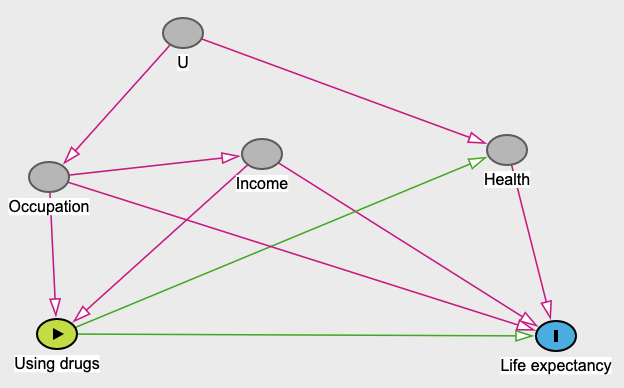
\includegraphics[width = \textwidth]{../img/drugs_dag1}

\end{frame}
% ----------------------------------------------------
\note{}

% ----------------------------------------------------
\begin{frame}
\frametitle{Front doors and back doors}
\centering

\begin{itemize}
  \item \texttt{Drugs > LifeExp}
  \item \texttt{Drugs > Health > LifeExp}
  \item \texttt{Drugs < Income > LifeExp}
  \item \texttt{Drugs < Occup > LifeExp}
  \item \texttt{Drugs < Occup > Income > LifeExp}
  \item \texttt{Drugs < Occup < U > Income > LifeExp}
  \item \texttt{Drugs < Occup < U > Health > LifeExp}
\end{itemize}

\end{frame}
% ----------------------------------------------------
\note{}

% ----------------------------------------------------
\begin{frame}
\frametitle{Front doors and back doors}
\centering

\begin{itemize}
  \item {\color{red}{\texttt{Drugs > LifeExp}}}
  \item {\color{red}{\texttt{Drugs > Health > LifeExp}}}
  \item \texttt{Drugs < Income > LifeExp}
  \item \texttt{Drugs < Occup > LifeExp}
  \item \texttt{Drugs < Occup > Income > LifeExp}
  \item \texttt{Drugs < Occup < U > Income > LifeExp}
  \item \texttt{Drugs < Occup < U > Health > LifeExp}
\end{itemize}

\end{frame}
% ----------------------------------------------------
\note{}

% ----------------------------------------------------
\begin{frame}
\frametitle{Front doors and back doors}
\centering

\begin{itemize}
  \item We just need to control for one of the variables in the path of a back door to close that path
  \item In this example, it would be enough to control for \texttt{income} and \texttt{occupation}
  \item This is the \textbf{back door criterion}
\end{itemize}

\end{frame}
% ----------------------------------------------------
\note{}

% ----------------------------------------------------
\begin{frame}
\frametitle{Front doors and back doors}
\centering

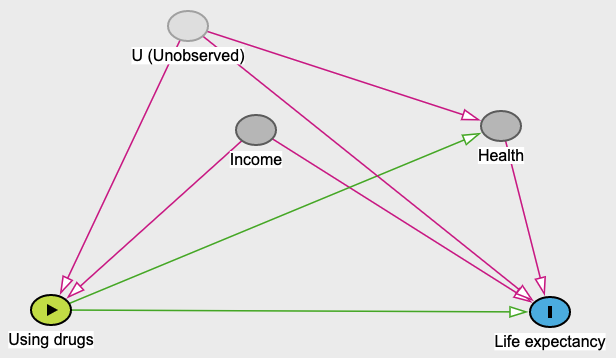
\includegraphics[width = \textwidth]{../img/drugs_dag2}

\end{frame}
% ----------------------------------------------------
\note{}

% ----------------------------------------------------
\begin{frame}
\frametitle{Front doors and back doors}
\centering

\begin{itemize}
  \item {\color{red}{\texttt{Drugs > LifeExp}}}
  \item {\color{red}{\texttt{Drugs > Health > LifeExp}}}
  \item \texttt{Drugs < Income > LifeExp}
  \item \texttt{Drugs < U > Income > LifeExp}
  \item \texttt{Drugs < U > Health > LifeExp}
  \item \texttt{Drugs < U > LifeExp}
\end{itemize}

\end{frame}
% ----------------------------------------------------
\note{}

% ----------------------------------------------------
\begin{frame}
\frametitle{Front doors and back doors}
\centering

\begin{itemize}
  \item \BGyellow{\textbf{What if we control for health?}}
  \item We would be blocking part of the causal `water flow' from drugs to life expectancy
  \item That's part of the mechanism: imagine that drugs has a direct effect, e.g. higher probability of dying on an accident, and an indirect effect through its effect on health
  \item (Unless you want to calculate the \textit{direct effect})
  \item[]
  \item<2-> We would have to control for \textbf{U}, which would close all other paths
\end{itemize}

\end{frame}
% ----------------------------------------------------
\note{}

% ----------------------------------------------------
\begin{frame}
\frametitle{Front doors and back doors}
\centering

\begin{itemize}
  \item {\color{red}{\texttt{Drugs > LifeExp}}}
  \item {\color{red}{\texttt{Drugs > Health > LifeExp}}}
  \item \texttt{Drugs < Income > LifeExp}
  \item \texttt{Drugs < U > Income > LifeExp}
  \item \texttt{Drugs < U > Health > LifeExp}
  \item \BGyellow{\texttt{Drugs < U > LifeExp}} \textbf{(!)}
  \item[]
  \item Problem? So?
\end{itemize}

\end{frame}
% ----------------------------------------------------
\note{}

% ----------------------------------------------------
\begin{frame}[fragile]
\frametitle{Off topic: Controlling}
\centering

\begin{itemize}
  \item How does alcohol consumption affect health?
  \item Imagine we take data from a group of people:
\end{itemize}

 \begin{lstlisting}[language=R]
df = data.frame(
  # In this group of people, one-third are rich
  rich = rbinom(500, 1, 0.3)) %>%
  # Rich people have 3x more money to buy whiskey
  mutate(whiskey = 3*rich + runif(500, 0, 4)) %>%
  # Health risk is worse if you drink more whiskey, but rich people have better health overall
  mutate(risk = -2*rich + 0.3*whiskey + rnorm(500, 2))
 \end{lstlisting}

\end{frame}
% ----------------------------------------------------
\note{}

% ----------------------------------------------------
\begin{frame}[fragile]
\frametitle{Off topic: Controlling}
\centering

\begin{lstlisting}[language=R]
cor(df$whiskey, df$risk)
[1] -0.1150553
\end{lstlisting}

\end{frame}
% ----------------------------------------------------
\note{}

% ----------------------------------------------------
\begin{frame}[fragile]
\frametitle{Off topic: Controlling}
\centering

\begin{itemize}
  \item Controlling for \texttt{rich} $=$ look at the variation \textbf{not} explained by \texttt{rich}
  \item i.e., take the group prediction out (mean of whiskey/risk for rich or non-rich)
\end{itemize}

\begin{lstlisting}[language=R]
df = df %>%
  group_by(rich) %>%
  mutate(whiskey_resid = whiskey - mean(whiskey),
         risk_resid = risk - mean(risk)) %>%
  ungroup()
\end{lstlisting}

\end{frame}
% ----------------------------------------------------
\note{}

% ----------------------------------------------------
\begin{frame}[fragile]
\frametitle{Off topic: Controlling}
\centering

\begin{itemize}
  \item The \textit{true} model we created:
  \item[] \texttt{risk = -2 * rich + .3 * whiskey + error}
\end{itemize}

\begin{lstlisting}[language=R]
cor(df$whiskey_resid, df$risk_resid)
[1] 0.3242735
\end{lstlisting}

\end{frame}
% ----------------------------------------------------
\note{}

% ====================================================
\section{Usual suspects}
% ====================================================

% ----------------------------------------------------
\begin{frame}
\frametitle{Usual suspects}
\centering

\begin{itemize}
  \item \hyperlink{confounding}{Confounding}
  \item \hyperlink{reverse}{Reverse causality}
  \item \hyperlink{bidirect}{Bidirectional causation}
  \item \hyperlink{selectbias}{Selection bias}
  \item \hyperlink{collider}{Collider bias}
  \item \hyperlink{ptbias}{Post-treatment bias}
\end{itemize}

\end{frame}
% ----------------------------------------------------
\note{}

% ----------------------------------------------------
\begin{frame}
\frametitle{Confounding}\label{confounding}
\centering

\begin{itemize}[<+->]
  \item Typical example: as the number of pirates in the oceans decreased, global mean temperature increased. Does it mean the disappearance of pirates is causing global warming?
  \item No, both are caused by the industrial revolution or technological development
  \item Months when people eat more ice-creams, also more people drown in the beach. Ice-creams causing drownings?
\end{itemize}

\end{frame}
% ----------------------------------------------------
\note{}

% ----------------------------------------------------
\begin{frame}
\frametitle{Reverse causality}\label{reverse}
\centering

\begin{itemize}
  \item Many examples where correlations we think imply a particular causal effect might be explained by its reverse: Violent videogames making teenagers violence? Drug use causes psychological problems?
  \item ``Hospitals make people sick.'' If you collect data on illness development, you might find that people fare worse if they go to the hospital. Obviously, it's a case of reverse causality: being sick causes going to the hospital.
\end{itemize}

\end{frame}
% ----------------------------------------------------
\note{}

% ----------------------------------------------------
\begin{frame}
\frametitle{Bidirectional causation}\label{bidirect}
\centering

\begin{itemize}
  \item (there are endogenous cycles, \textit{not the same as} reverse causality)
  \item[]
  \item Political values and voting: they way you think makes you vote in a particular way, but the way you vote can also affect the way you think (group influence, cognitive processes, etc)
  \item Can be closely related to selection bias: imagine we go to Madrid Rio and we measure if people doing exercises are more likely to be overweight than those lying around
  \item We probably don't find any result. Does it mean exercise does not decrease overweight? No, it's probably bidirectional causation: overweight makes people more likely to exercise, and exercise reduces overweight
\end{itemize}

\end{frame}
% ----------------------------------------------------
\note{}

% ----------------------------------------------------
\begin{frame}
\frametitle{}
\centering

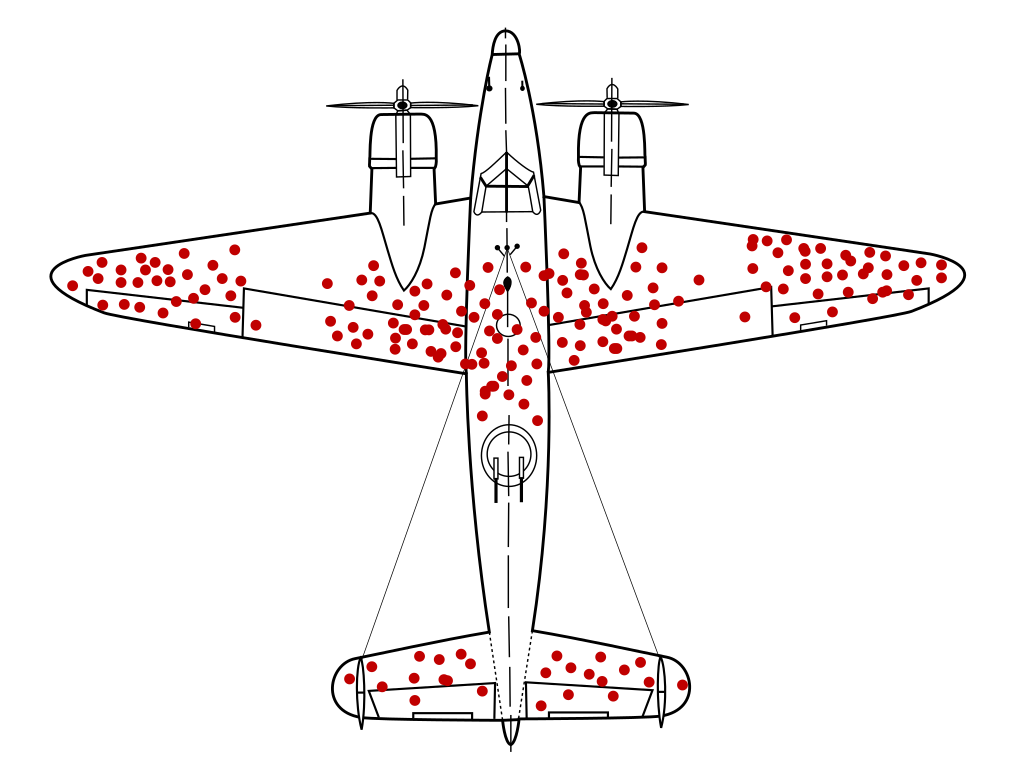
\includegraphics[width = 0.8\textwidth]{../img/Survivorship-bias}

\end{frame}
% ----------------------------------------------------
\note{}

% ----------------------------------------------------
\begin{frame}
\frametitle{Selection bias}\label{selectbias}
\centering

\begin{itemize}
  \item Our observations are not representative
  \item Famous example from World War II airplanes
  \item Many examples: advice from successful CEOs, ex-heroin addicts more likely to do sports, etc
  \item Why?
  \begin{itemize}
    \item Sampling
    \item Attrition ($\approx$ survivorship bias)
    \item etc
  \end{itemize}
\end{itemize}

\end{frame}
% ----------------------------------------------------
\note{}
% ----------------------------------------------------
\begin{frame}
\frametitle{Selection bias in causal inference}
\centering

\begin{itemize}
  \item Selection bias in statistics: sampling issue
  \item Quite different in causality: we're dealing with \BGyellow{selection into treatment}
  % \item Remember example from HIV treatments studies
\end{itemize}

\end{frame}
% ----------------------------------------------------
\note{}

% ----------------------------------------------------
\begin{frame}
\frametitle{Collider bias}\label{collider}
\centering

\begin{tikzpicture}
% nodes %
\node (Y) at (2,0){Outcome};
\node (D) at (-2,0){Treatment};
\node (U) at (0,3){Z};
\draw[->] (D) -- (Y);
\draw[<-] (U) -- (D);
\draw[<-] (U) -- (Y);
\end{tikzpicture}

\end{frame}
% ----------------------------------------------------
\note{}

% % ----------------------------------------------------
% \begin{frame}
% \frametitle{Collider bias}
% \centering
%
% 
\includegraphics[width = 0.7\textwidth]{../img/crazyhot}
%
% \end{frame}
% % ----------------------------------------------------

% ----------------------------------------------------
\begin{frame}[fragile]
\frametitle{Collider bias}
\centering

\begin{itemize}
  \item Do smart people lack social skills?
  \item We have 1,000 people, with \textbf{randomly} distributed intelligence and social skills
\end{itemize}

 \begin{lstlisting}[language=R]
 set.seed(7891234)
 df = data.frame(
   intelligence = rnorm(1000, mean = 5, sd = 1.5),
   social_skills = rnorm(1000, mean = 5, sd = 1.5))
 \end{lstlisting}

\end{frame}
% ----------------------------------------------------
\note{}

% ----------------------------------------------------
\begin{frame}[fragile]
\frametitle{Collider bias}
\centering

\begin{itemize}
  \item No correlation
\end{itemize}

 \begin{lstlisting}[language=R]
 > cor(df$intelligence, df$social_skills)
 [1] -0.03982793
 \end{lstlisting}

\end{frame}
% ----------------------------------------------------
\note{}

% ----------------------------------------------------
\begin{frame}
\frametitle{Collider bias}
\centering

\begin{itemize}
  \item Now imagine that we have another variable, the probability of being hired in a company, which is caused by both intelligence and social skills:
\end{itemize}

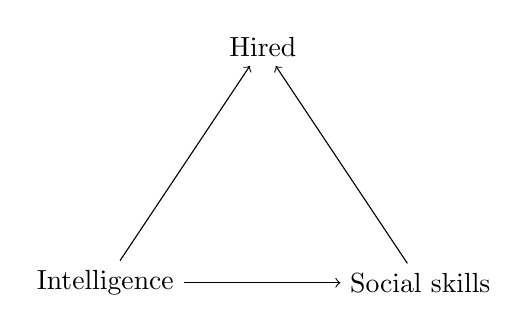
\begin{tikzpicture}
% nodes %
\node (Y) at (2,0){Social skills};
\node (D) at (-2,0){Intelligence};
\node (U) at (0,3){Hired};
\draw[->] (D) -- (Y);
\draw[<-] (U) -- (D);
\draw[<-] (U) -- (Y);
\end{tikzpicture}

\end{frame}
% ----------------------------------------------------
\note{}

% ----------------------------------------------------
\begin{frame}[fragile]
\frametitle{Collider bias}
\centering

\begin{itemize}
  \item This company values intelligence a bit more, but takes both into account. And hires the 25\% best candidates:
\end{itemize}

\begin{lstlisting}[language=R]
  df = df %>%
    mutate(
      points = 3 * intelligence + 2 * social_skills) %>%
    mutate(hired_binary =
      ifelse(points > quantile(points, 0.75), 1, 0))
\end{lstlisting}

\end{frame}
% ----------------------------------------------------
\note{}

% ----------------------------------------------------
\begin{frame}[plain]
  \begin{tikzpicture}[remember picture, overlay]
    \node[at = (current page.center), yshift = 0cm] (cover) {%
      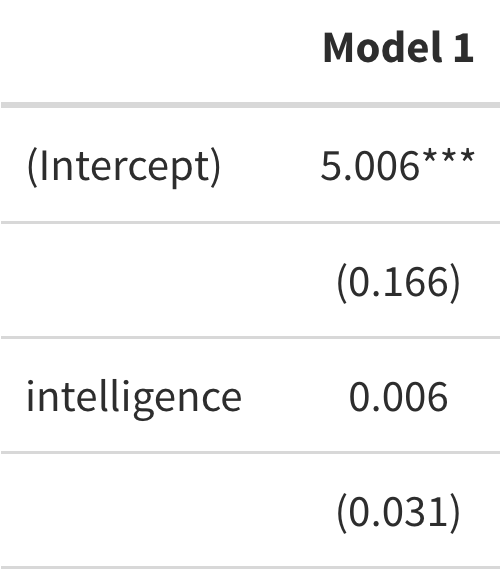
\includegraphics[keepaspectratio, width=\paperwidth, height=\paperheight]{../img/collider_m1}};
  \end{tikzpicture}
\end{frame}
% ----------------------------------------------------
\note{}

% ----------------------------------------------------
\begin{frame}[plain]
  \begin{tikzpicture}[remember picture, overlay]
    \node[at = (current page.center), yshift = 0cm] (cover) {%
      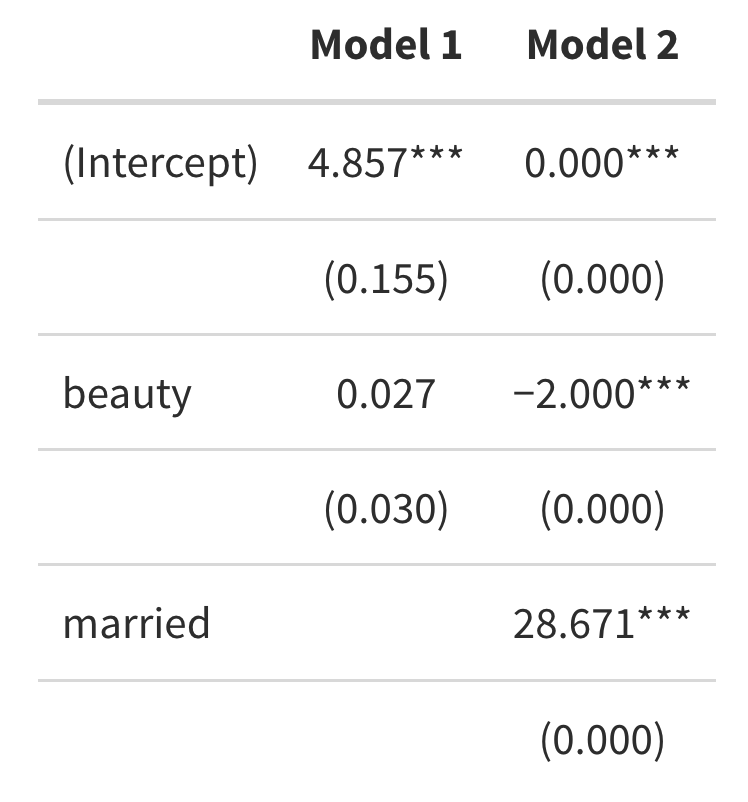
\includegraphics[keepaspectratio, width=\paperwidth, height=\paperheight]{../img/collider_m2}};
  \end{tikzpicture}
\end{frame}
% ----------------------------------------------------
\note{}

% ----------------------------------------------------
\begin{frame}[plain]
  \begin{tikzpicture}[remember picture, overlay]
    \node[at = (current page.center), yshift = 0cm] (cover) {%
      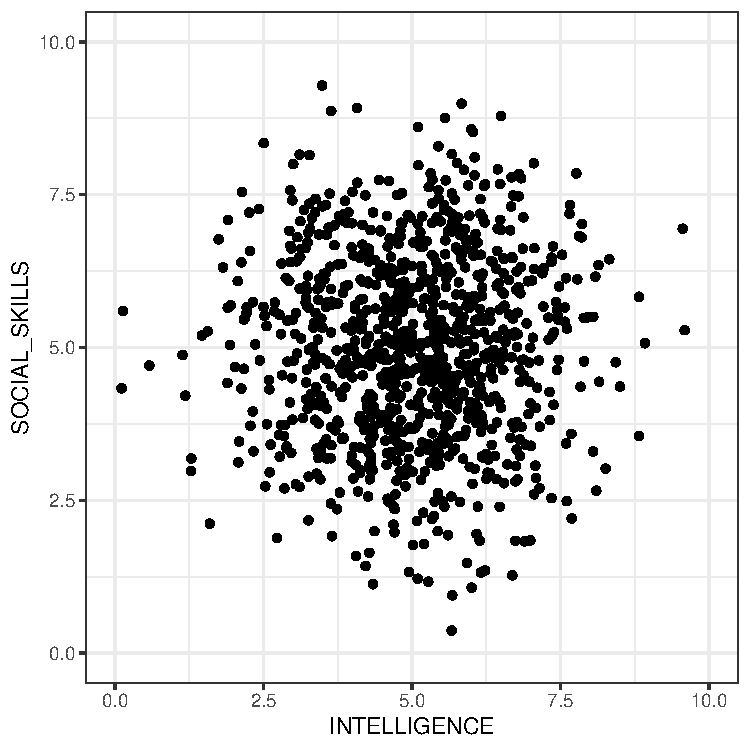
\includegraphics[keepaspectratio, width=\paperwidth, height=\paperheight]{../img/collider1}};
  \end{tikzpicture}
\end{frame}
% ----------------------------------------------------
\note{}

% ----------------------------------------------------
\begin{frame}[plain]
  \begin{tikzpicture}[remember picture, overlay]
    \node[at = (current page.center), yshift = 0cm] (cover) {%
      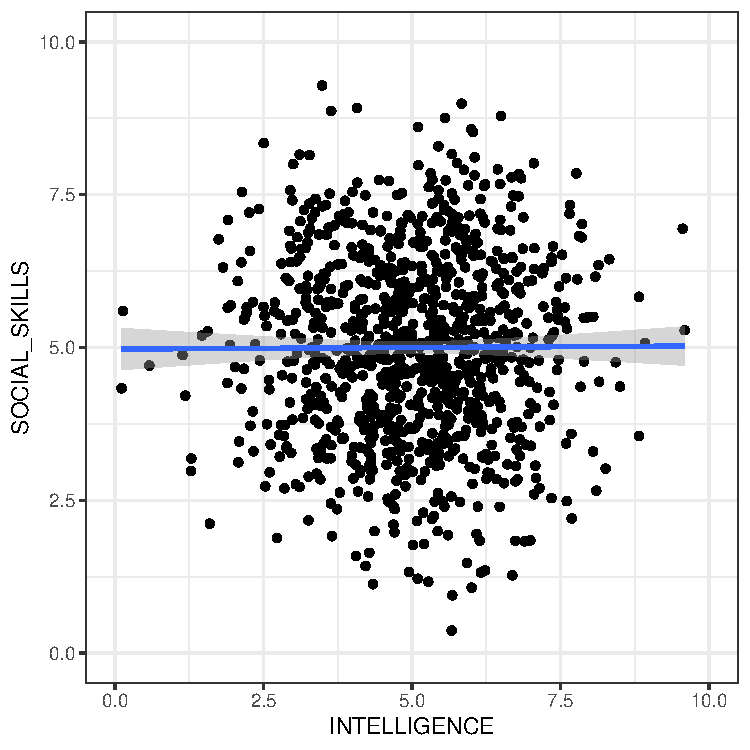
\includegraphics[keepaspectratio, width=\paperwidth, height=\paperheight]{../img/collider2}};
  \end{tikzpicture}
\end{frame}
% ----------------------------------------------------
\note{}

% ----------------------------------------------------
\begin{frame}[plain]
  \begin{tikzpicture}[remember picture, overlay]
    \node[at = (current page.center), yshift = 0cm] (cover) {%
      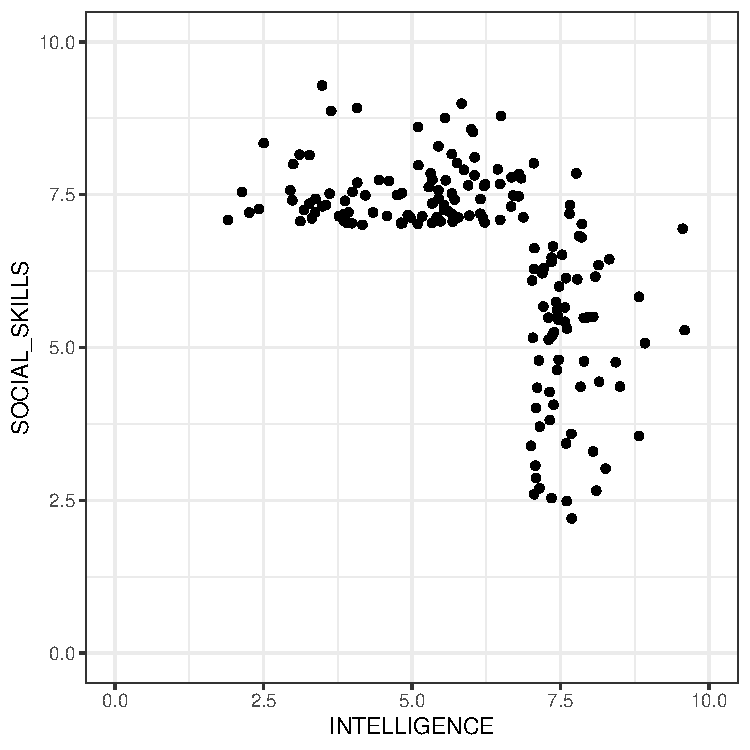
\includegraphics[keepaspectratio, width=\paperwidth, height=\paperheight]{../img/collider3}};
  \end{tikzpicture}
\end{frame}
% ----------------------------------------------------
\note{}

% ----------------------------------------------------
\begin{frame}[plain]
  \begin{tikzpicture}[remember picture, overlay]
    \node[at = (current page.center), yshift = 0cm] (cover) {%
      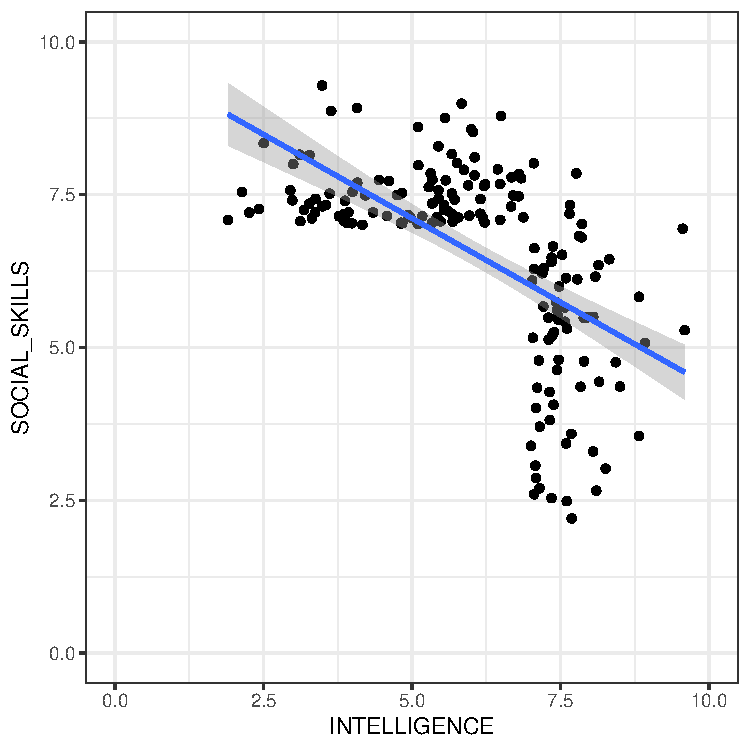
\includegraphics[keepaspectratio, width=\paperwidth, height=\paperheight]{../img/collider4}};
  \end{tikzpicture}
\end{frame}
% ----------------------------------------------------
\note{}

% ----------------------------------------------------
\begin{frame}[plain]
  \begin{tikzpicture}[remember picture, overlay]
    \node[at = (current page.center), yshift = 0cm] (cover) {%
      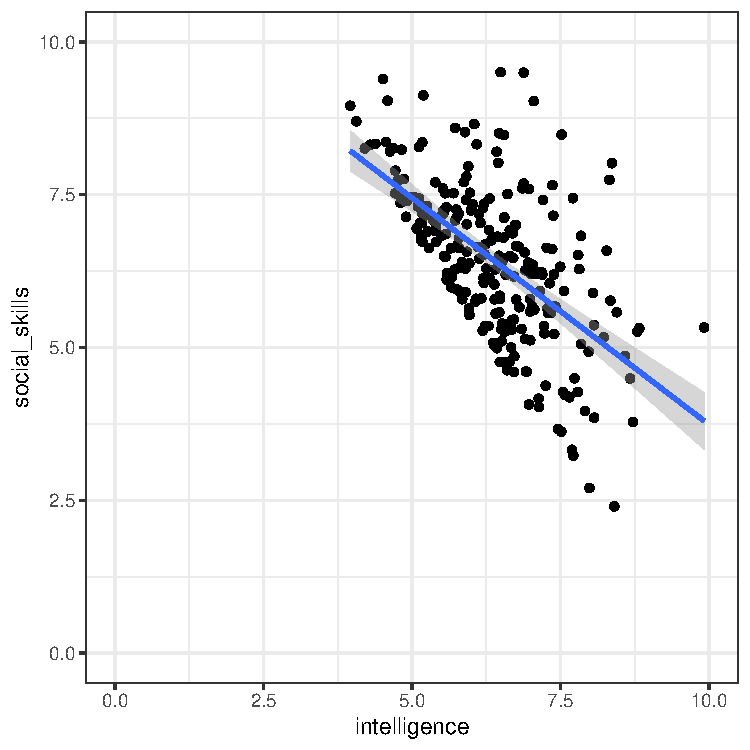
\includegraphics[keepaspectratio, width=\paperwidth, height=\paperheight]{../img/collider5}};
  \end{tikzpicture}
\end{frame}
% ----------------------------------------------------
\note{}

% ----------------------------------------------------
\begin{frame}
\frametitle{Collider bias}
\centering

\begin{itemize}
  \item A collider bias \textbf{opens} a path when you control for the variable
\end{itemize}

\end{frame}
% ----------------------------------------------------
\note{}

% ----------------------------------------------------
\begin{frame}
\frametitle{Collider bias}
\centering

\begin{minipage}{.54\textwidth}\centering
\begin{itemize}
  \item Another example in life sciences where we can only use observational data, the `obesity paradox'
  \begin{itemize}
    \item Obesity reduces mortality among patients with some chronic heart diseases
  \end{itemize}
  \item Collider bias?
  \begin{itemize}
    \item \url{https://catalogofbias.org/biases/collider-bias/}
  \end{itemize}
\end{itemize}
\end{minipage}\hfill
\begin{minipage}{0.45\textwidth}\centering
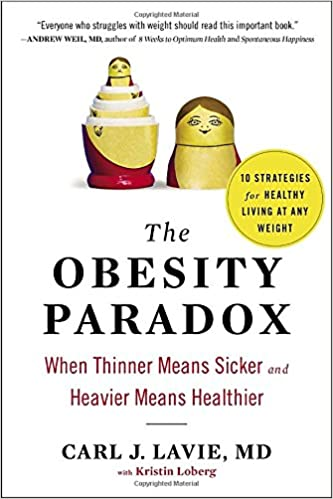
\includegraphics[width = 0.9\textwidth]{../img/obesity_paradox}
\end{minipage}

\end{frame}
% ----------------------------------------------------
\note{}

% ----------------------------------------------------
\begin{frame}
\frametitle{Collider bias}
\centering

\begin{itemize}
  \item Animated: \url{https://nickchk.com/causalgraphs.html}
\end{itemize}

\end{frame}
% ----------------------------------------------------
\note{}

% ----------------------------------------------------
\begin{frame}
\frametitle{Post-treatment bias (collider again)}\label{ptbias}
\centering

\begin{itemize}[<+->]
  \item We want to know whether suffering violence during a civil wars makes people more or less likely to support certain authorities decades after the war
  \item And we say: well, the country develop economically after the war, so maybe it makes sense to control for local increase in GDPpc, because it will also affect support
\end{itemize}

\end{frame}
% ----------------------------------------------------
\note{}

% ----------------------------------------------------
\begin{frame}
\frametitle{Nice try, but...}
\centering

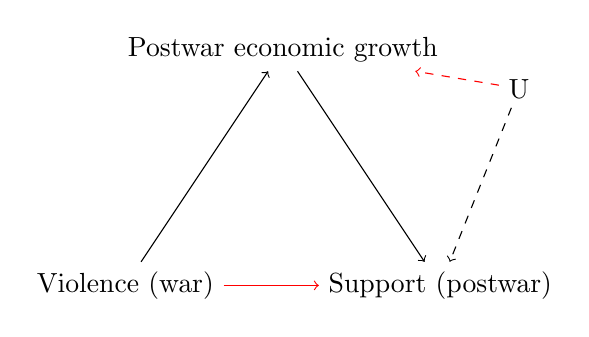
\begin{tikzpicture}
% nodes %
\node (Y) at (2,0){Support (postwar)};
\node (D) at (-2,0){Violence (war)};
\node (Z) at (0,3){Postwar economic growth};
\node (U) at (3,2.5){\BGyellow{U}};
\draw[->, red] (D) -- (Y);
\draw[<-] (Z) -- (D);
\draw[->] (Z) -- (Y);
\draw[->, dashed, red] (U) -- (Z);
\draw[->, dashed] (U) -- (Y);
\end{tikzpicture}

\end{frame}
% ----------------------------------------------------
\note{}

% ----------------------------------------------------
\begin{frame}
\frametitle{Recap: what should \BGyellow{not} be controlled for}
\centering

\begin{itemize}
  \item[1.] \BGyellow{Front-door paths}
  \begin{itemize}
    \item Blocking some of the effect through a mediator variable
    \item (There are almost always mediator variables, so you could potentially just eliminate all the effect you're trying to identify)
  \end{itemize}
  \item[]
  \item[2.] \BGyellow{Collider bias}
  \begin{itemize}
    \item Opens a new, uncontrolled-for path
    \item Sometimes you might be inadvertently controlling for a collider because of \textit{selection} issues
    \item Extra care with post-treatment bias
  \end{itemize}
\end{itemize}

\end{frame}
% ----------------------------------------------------
\note{}

% ====================================================
\section{Paper: Guess et al.\ (2023)}
% ====================================================

% ----------------------------------------------------
\begin{frame}[plain]
  \begin{tikzpicture}[remember picture, overlay]
    \node[at = (current page.center), yshift = 0cm] (cover) {%
      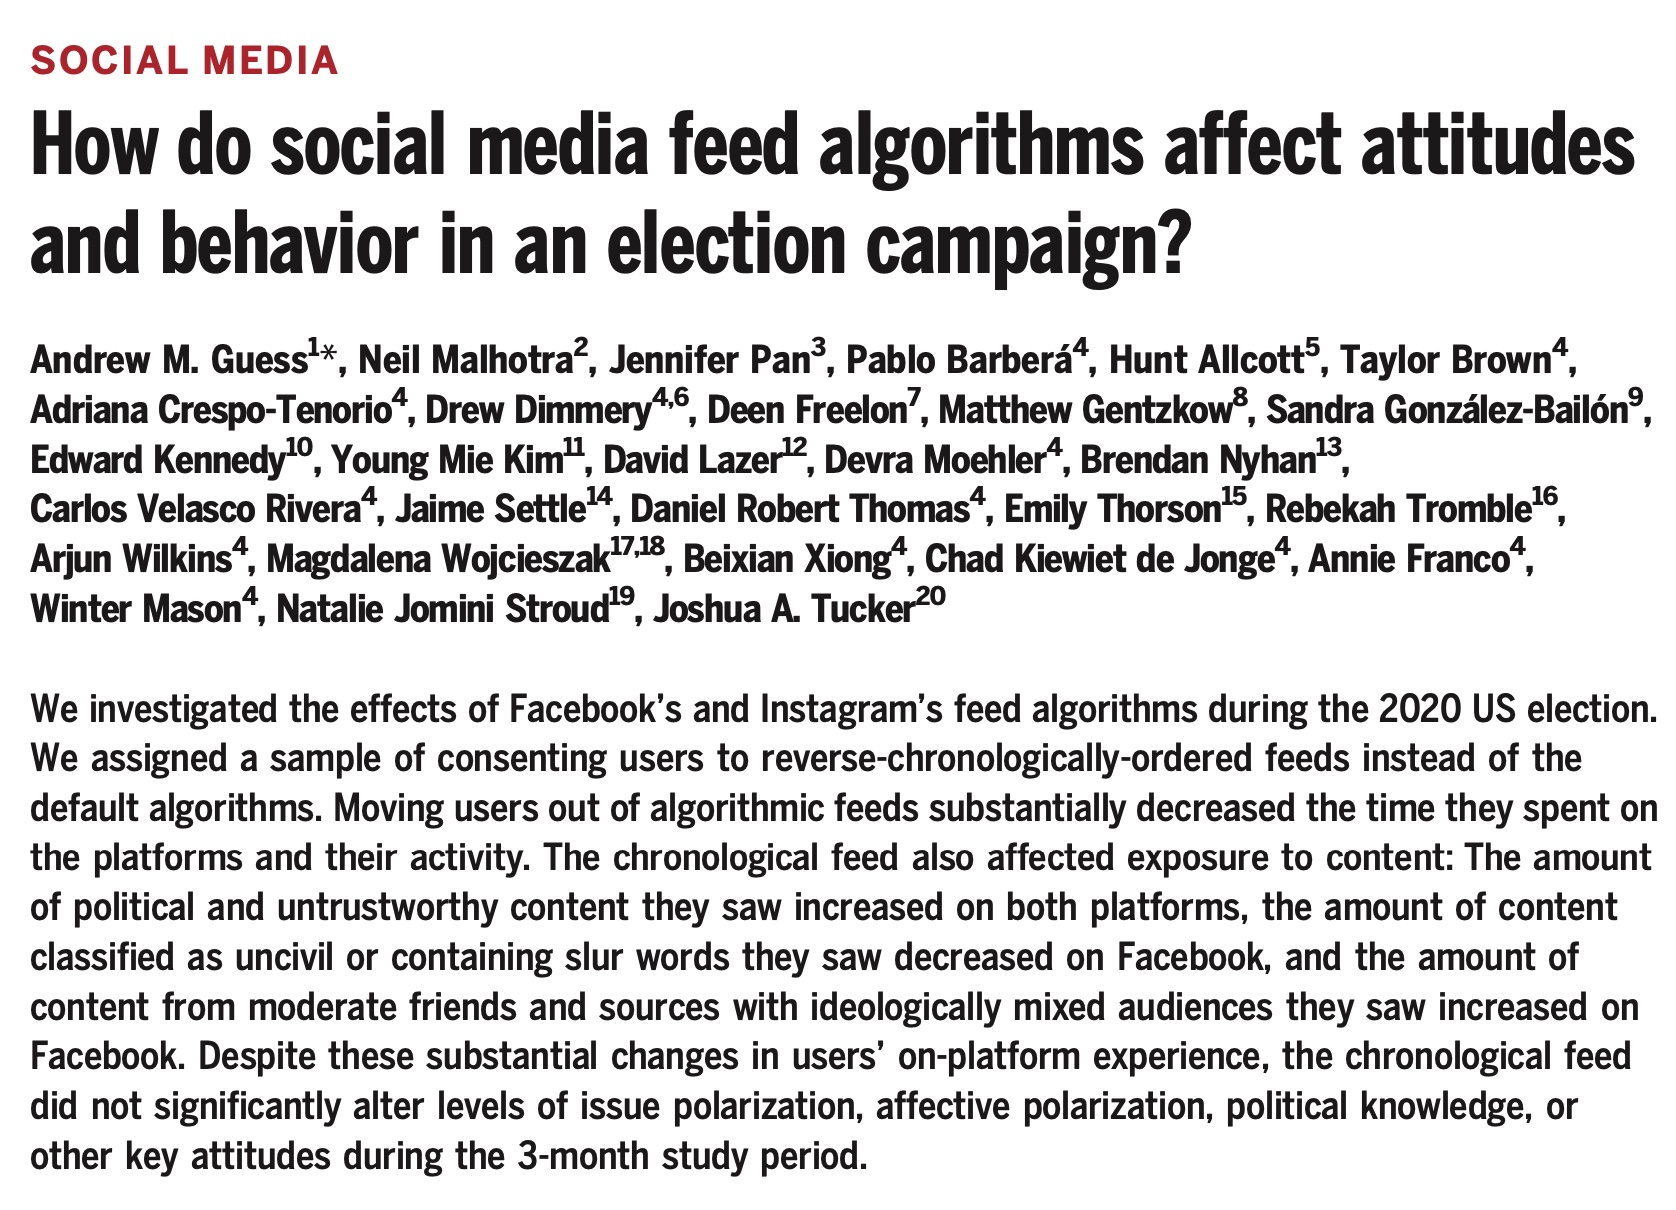
\includegraphics[keepaspectratio, width=.95\paperwidth, height=.9\paperheight]{../img/guess2023}};
  \end{tikzpicture}
\end{frame}
% ----------------------------------------------------
\note{One minute of summary. Facebook and Instagram users who consented were randomly switched to a chronological feed for three months of the 2020 US campaign.

The feed changed a lot: less time on the platforms, more political content, more untrustworthy content, less incivility. Attitudes barely moved: polarization, knowledge and other outcomes showed no significant change.

Worth noting the collaboration model: academics with Meta, with pre-registered analyses. It is part of why the results are credible and part of the access story from week 2.}

% ----------------------------------------------------
\begin{frame}
\frametitle{In pairs/groups}
\centering

\vspace{10pt}
\begin{itemize}
  \item[1.] What exactly was \textbf{randomized}, and what was not?
  \vspace{8pt}
  \item[2.] \textbf{Who consented}, and how does that bound the estimate?
  \vspace{8pt}
  \item[3.] The effect is near zero. What have we learned: about \textbf{feeds}, or about \textbf{three months}?
  \vspace{8pt}
  \item[4.] Where does \textbf{SUTVA} fail here?
\end{itemize}

\end{frame}
% ----------------------------------------------------
\note{Twelve minutes: 1 and 2 together, then 3 and 4.

\begin{itemize}
  \item[1.] The feed order of the participant. Not their friends' feeds, not what gets produced on the platform, not the rest of their media diet.
  \item[2.] People who accepted an invitation in their feed and agreed to be studied. Probably more interested in politics and more trusting of research. The estimate is for them.
  \item[3.] Both are open. Three months at the end of a saturated campaign is a hard place to move anyone. A null here is not evidence that feeds never matter.
  \item[4.] SUTVA proper: treated users share differently, which changes their friends' feeds. Related but distinct: scale (years of algorithmic feeds for everyone shaped the ecosystem, and one person's switch does not undo that) and substitution (treated users moved time to other apps, a bundled treatment).
\end{itemize}}

% ----------------------------------------------------
\begin{frame}
\frametitle{Groups of four: design the next one}
\centering

\vspace{20pt}
{\large You get the same access, and one year.}

\vspace{12pt}
{\large What would you change so that\\a null result would tell you more?}

\end{frame}
% ----------------------------------------------------
\note{Seven minutes, then three groups report back. Same move as weeks 2 and 3.

Good answers: run it longer, or outside an election; randomize at the level of friendship clusters or whole communities; measure behaviour (sharing, voting) as well as attitudes; recruit to reduce consent-based selection, or measure how participants differ from users; track time moved to other platforms.

Push on the trade-offs: every one of those costs something, often the ethics or the access.}

% ====================================================
\section{Before next week}
% ====================================================

% ----------------------------------------------------
\begin{frame}
\frametitle{The three goals, after today}
\centering

\vspace{10pt}
\begin{itemize}
  \item \textbf{Describe}: not every relationship needs a cause. Say which you have
  \vspace{8pt}
  \item \textbf{Explain}: every causal claim is a comparison. Name it
  \vspace{8pt}
  \item \textbf{Predict}: good prediction needs no identification, and gives none
\end{itemize}

\end{frame}
% ----------------------------------------------------
\note{One line per goal. The middle one is Memo 4.

Close the loop on the opener: which comparison would pick among the three stories behind the infant mortality plot?}

% ----------------------------------------------------
\begin{frame}
\frametitle{Next week}
\centering

\vspace{25pt}
{\large Today: close the back doors.\\[6pt] Next week: find variation where they are closed \textbf{by design}.}

\end{frame}
% ----------------------------------------------------
\note{Hand over to week 5: DiD, RDD, IV and friends, each as a way of finding a credible stand-in for Gary. Then: how far results travel, and how to keep yourself honest.}

% ----------------------------------------------------
\begin{frame}
\frametitle{Before next week}
\centering

\vspace{8pt}
\begin{itemize}
  \item \textbf{No reading}. Use the time for Memo 4, and your group
  \vspace{12pt}
  \item<2-> \textbf{Memo 4}, in pairs, Aula Global by \textbf{Monday night}:
  \begin{itemize}
    \item<2-> Take a causal claim from the news or a paper
    \item<2-> What comparison would license it? Draw the DAG
    \item<2-> Which usual suspect would bias it most?
    \item<2-> Half a page (plus the diagram)
  \end{itemize}
  \vspace{12pt}
  \item<3-> Workshop groups are fixed by \textbf{Mon Oct 19}, with Memo 5
\end{itemize}

\end{frame}
% ----------------------------------------------------
\note{Memo 4 is today applied to a claim they choose. Push them towards claims they actually care about; news headlines of the form ``X linked to Y'' are ideal material.

The diagram is the heart of it. A photo of a hand drawing is fine. What matters is that every arrow is a claim and every missing arrow is a claim.

Remind them about groups: whoever submits Memo 5 together on Oct 19 presents together and writes the essay together. If they have not started talking to people, this week is the moment.}

% ----------------------------------------------------
\begin{frame}
\frametitle{}
\centering

\vspace{40pt}
{\Large Questions?}

\end{frame}
% ----------------------------------------------------
\note{}
